\documentclass[a4paper]{book}
\usepackage{a4wide}
\usepackage{makeidx}
\usepackage{graphicx}
\usepackage{multicol}
\usepackage{float}
\usepackage{listings}
\usepackage{color}
\usepackage{textcomp}
\usepackage{alltt}
\usepackage{times}
\usepackage[utf8]{inputenc}
\usepackage{doxygen}
\lstset{language=C++,inputencoding=utf8,basicstyle=\footnotesize,breaklines=true,breakatwhitespace=true,tabsize=8,numbers=left }
\makeindex
\setcounter{tocdepth}{3}
\renewcommand{\footrulewidth}{0.4pt}
\begin{document}
\begin{titlepage}
\vspace*{7cm}
\begin{center}
{\Large MarsinEngine \\[1ex]\large Iteration1 }\\
\vspace*{1cm}
{\large Generated by Doxygen 1.7.1}\\
\vspace*{0.5cm}
{\small Mon Oct 31 2011 13:41:24}\\
\end{center}
\end{titlepage}
\clearemptydoublepage
\pagenumbering{roman}
\tableofcontents
\clearemptydoublepage
\pagenumbering{arabic}
\chapter{Class Index}
\section{Class Hierarchy}
This inheritance list is sorted roughly, but not completely, alphabetically:\begin{DoxyCompactList}
\item \contentsline{section}{Engine.Collision.CollisionEvent}{\pageref{class_engine_1_1_collision_1_1_collision_event}}{}
\item \contentsline{section}{Engine.Collision.CollisionListener}{\pageref{interface_engine_1_1_collision_1_1_collision_listener}}{}
\begin{DoxyCompactList}
\item \contentsline{section}{Engine.Collision.CollisionAdapter}{\pageref{class_engine_1_1_collision_1_1_collision_adapter}}{}
\end{DoxyCompactList}
\item \contentsline{section}{Engine.EngineStarter}{\pageref{class_engine_1_1_engine_starter}}{}
\item \contentsline{section}{Engine.Forces.Force}{\pageref{class_engine_1_1_forces_1_1_force}}{}
\begin{DoxyCompactList}
\item \contentsline{section}{Engine.Forces.Weight}{\pageref{class_engine_1_1_forces_1_1_weight}}{}
\item \contentsline{section}{Engine.Forces.Wind}{\pageref{class_engine_1_1_forces_1_1_wind}}{}
\end{DoxyCompactList}
\item \contentsline{section}{Test.IterationOneTestApplication}{\pageref{class_test_1_1_iteration_one_test_application}}{}
\item \contentsline{section}{Engine.Utilities.Line2D}{\pageref{class_engine_1_1_utilities_1_1_line2_d}}{}
\item \contentsline{section}{Engine.Objects.Object2D}{\pageref{class_engine_1_1_objects_1_1_object2_d}}{}
\begin{DoxyCompactList}
\item \contentsline{section}{Engine.Objects.CircularObject}{\pageref{class_engine_1_1_objects_1_1_circular_object}}{}
\item \contentsline{section}{Engine.Objects.RectangularObject}{\pageref{class_engine_1_1_objects_1_1_rectangular_object}}{}
\end{DoxyCompactList}
\item \contentsline{section}{Engine.Utilities.Point2D}{\pageref{class_engine_1_1_utilities_1_1_point2_d}}{}
\item \contentsline{section}{Engine.Properties}{\pageref{interface_engine_1_1_properties}}{}
\item \contentsline{section}{Test.TestApp1}{\pageref{class_test_1_1_test_app1}}{}
\item \contentsline{section}{Engine.Utilities.Vector2D}{\pageref{class_engine_1_1_utilities_1_1_vector2_d}}{}
\item \contentsline{section}{Engine.Objects.ObjectAttributes.Velocity}{\pageref{class_engine_1_1_objects_1_1_object_attributes_1_1_velocity}}{}
\item \contentsline{section}{Engine.World.World}{\pageref{class_engine_1_1_world_1_1_world}}{}
\end{DoxyCompactList}

\chapter{Class Index}
\section{Class List}
Here are the classes, structs, unions and interfaces with brief descriptions:\begin{DoxyCompactList}
\item\contentsline{section}{{\bf Engine.Objects.CircularObject} }{\pageref{class_engine_1_1_objects_1_1_circular_object}}{}
\item\contentsline{section}{{\bf Engine.Collision.CollisionAdapter} }{\pageref{class_engine_1_1_collision_1_1_collision_adapter}}{}
\item\contentsline{section}{{\bf Engine.Collision.CollisionEvent} }{\pageref{class_engine_1_1_collision_1_1_collision_event}}{}
\item\contentsline{section}{{\bf Engine.Collision.CollisionListener} }{\pageref{interface_engine_1_1_collision_1_1_collision_listener}}{}
\item\contentsline{section}{{\bf Engine.EngineStarter} }{\pageref{class_engine_1_1_engine_starter}}{}
\item\contentsline{section}{{\bf Engine.Forces.Force} }{\pageref{class_engine_1_1_forces_1_1_force}}{}
\item\contentsline{section}{{\bf Test.IterationOneTestApplication} }{\pageref{class_test_1_1_iteration_one_test_application}}{}
\item\contentsline{section}{{\bf Engine.Utilities.Line2D} }{\pageref{class_engine_1_1_utilities_1_1_line2_d}}{}
\item\contentsline{section}{{\bf Engine.Objects.Object2D} }{\pageref{class_engine_1_1_objects_1_1_object2_d}}{}
\item\contentsline{section}{{\bf Engine.Utilities.Point2D} }{\pageref{class_engine_1_1_utilities_1_1_point2_d}}{}
\item\contentsline{section}{{\bf Engine.Properties} }{\pageref{interface_engine_1_1_properties}}{}
\item\contentsline{section}{{\bf Engine.Objects.RectangularObject} }{\pageref{class_engine_1_1_objects_1_1_rectangular_object}}{}
\item\contentsline{section}{{\bf Test.TestApp1} }{\pageref{class_test_1_1_test_app1}}{}
\item\contentsline{section}{{\bf Engine.Utilities.Vector2D} }{\pageref{class_engine_1_1_utilities_1_1_vector2_d}}{}
\item\contentsline{section}{{\bf Engine.Objects.ObjectAttributes.Velocity} }{\pageref{class_engine_1_1_objects_1_1_object_attributes_1_1_velocity}}{}
\item\contentsline{section}{{\bf Engine.Forces.Weight} }{\pageref{class_engine_1_1_forces_1_1_weight}}{}
\item\contentsline{section}{{\bf Engine.Forces.Wind} }{\pageref{class_engine_1_1_forces_1_1_wind}}{}
\item\contentsline{section}{{\bf Engine.World.World} }{\pageref{class_engine_1_1_world_1_1_world}}{}
\end{DoxyCompactList}

\chapter{Class Documentation}
\section{Engine.Objects.CircularObject Class Reference}
\label{class_engine_1_1_objects_1_1_circular_object}\index{Engine::Objects::CircularObject@{Engine::Objects::CircularObject}}
Inheritance diagram for Engine.Objects.CircularObject:\begin{figure}[H]
\begin{center}
\leavevmode
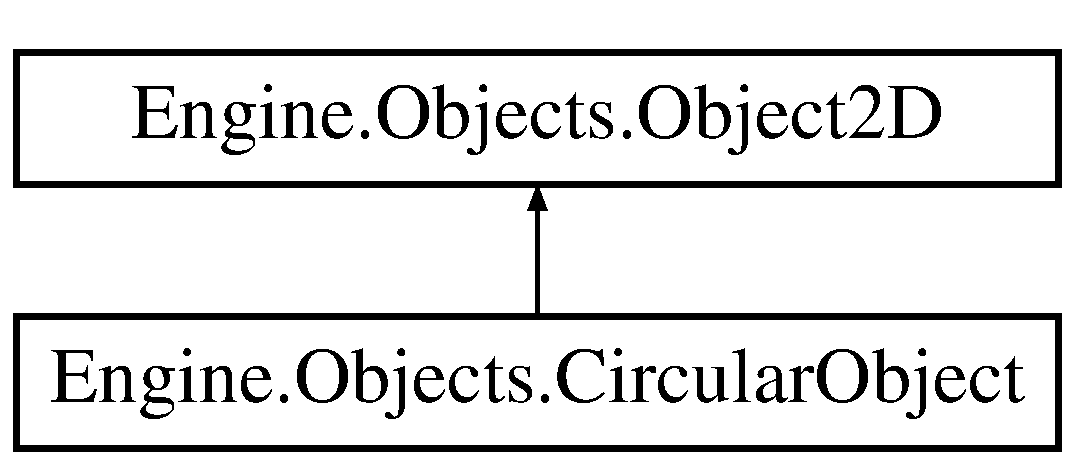
\includegraphics[height=2.000000cm]{class_engine_1_1_objects_1_1_circular_object}
\end{center}
\end{figure}
\subsection*{Public Member Functions}
\begin{DoxyCompactItemize}
\item 
{\bf CircularObject} ()
\item 
{\bf CircularObject} (int a, int b)
\item 
{\bf CircularObject} (double mass, {\bf Point2D} location, double fi, {\bf Velocity} velocity, int a, int b)
\item 
int {\bf getA} ()
\item 
void {\bf setA} (int a)
\item 
int {\bf getB} ()
\item 
void {\bf setB} (int b)
\item 
{\bf Point2D} {\bfseries getCenter} ()\label{class_engine_1_1_objects_1_1_circular_object_a154e248dce79ba14bdb9ba0d377235ec}

\item 
void {\bfseries setCenter} ({\bf Point2D} center)\label{class_engine_1_1_objects_1_1_circular_object_a824b3808845ee9afcd8bee341bb08b11}

\item 
void {\bfseries updateCenter} ()\label{class_engine_1_1_objects_1_1_circular_object_ae651728538199280364efa7e1e96576e}

\end{DoxyCompactItemize}
\subsection*{Package Attributes}
\begin{DoxyCompactItemize}
\item 
int {\bfseries a} = 100\label{class_engine_1_1_objects_1_1_circular_object_a36457cf37cac53dd7cf072a76219ea55}

\item 
int {\bfseries b} = 100\label{class_engine_1_1_objects_1_1_circular_object_ab07878d2a49b18210c6d8e1d2268c1b1}

\item 
{\bf Point2D} {\bfseries center}\label{class_engine_1_1_objects_1_1_circular_object_abed3c114e7e777a41be8a484f5230ee0}

\end{DoxyCompactItemize}


\subsection{Detailed Description}
Created by IntelliJ IDEA. User: Sina Solaimanpour Date: 10/18/11 Time: 10:40 PM 

\subsection{Constructor \& Destructor Documentation}
\index{Engine::Objects::CircularObject@{Engine::Objects::CircularObject}!CircularObject@{CircularObject}}
\index{CircularObject@{CircularObject}!Engine::Objects::CircularObject@{Engine::Objects::CircularObject}}
\subsubsection[{CircularObject}]{\setlength{\rightskip}{0pt plus 5cm}Engine.Objects.CircularObject.CircularObject (
\begin{DoxyParamCaption}
{}
\end{DoxyParamCaption}
)}\label{class_engine_1_1_objects_1_1_circular_object_a703d513c6a40fb72294759d6ed1af8a8}
Default Constructor, It sets a = 100, and b = 100 Which it creates a Circle With 2R = 100 \index{Engine::Objects::CircularObject@{Engine::Objects::CircularObject}!CircularObject@{CircularObject}}
\index{CircularObject@{CircularObject}!Engine::Objects::CircularObject@{Engine::Objects::CircularObject}}
\subsubsection[{CircularObject}]{\setlength{\rightskip}{0pt plus 5cm}Engine.Objects.CircularObject.CircularObject (
\begin{DoxyParamCaption}
\item[{int}]{ a, }
\item[{int}]{ b}
\end{DoxyParamCaption}
)}\label{class_engine_1_1_objects_1_1_circular_object_a8a7bd04d778f36a3cf29cedab2798863}
It Creates a Circular object with A = a, and B = b if you pass values which a == b it will create a circle with 2R == a == b other properties will be set to a default value preset. (For More Info Read in Object2D's Page...)


\begin{DoxyParams}{Parameters}
\item[{\em a}]Width of the Circular Object \item[{\em b}]Height og the Circular Object \end{DoxyParams}
\index{Engine::Objects::CircularObject@{Engine::Objects::CircularObject}!CircularObject@{CircularObject}}
\index{CircularObject@{CircularObject}!Engine::Objects::CircularObject@{Engine::Objects::CircularObject}}
\subsubsection[{CircularObject}]{\setlength{\rightskip}{0pt plus 5cm}Engine.Objects.CircularObject.CircularObject (
\begin{DoxyParamCaption}
\item[{double}]{ mass, }
\item[{{\bf Point2D}}]{ location, }
\item[{double}]{ fi, }
\item[{{\bf Velocity}}]{ velocity, }
\item[{int}]{ a, }
\item[{int}]{ b}
\end{DoxyParamCaption}
)}\label{class_engine_1_1_objects_1_1_circular_object_a38cd1eda3c96edadd3f67521a45626d7}
Main Constructor for the Circular Objects


\begin{DoxyParams}{Parameters}
\item[{\em mass}]Object's Mass \item[{\em location}]Object's Location \item[{\em fi}]Object's Rotation Angle (in Degrees) \item[{\em velocity}]Object's Initial Velocity \item[{\em a}]Width of the Circular Object \item[{\em b}]Height og the Circular Object \end{DoxyParams}


\subsection{Member Function Documentation}
\index{Engine::Objects::CircularObject@{Engine::Objects::CircularObject}!getA@{getA}}
\index{getA@{getA}!Engine::Objects::CircularObject@{Engine::Objects::CircularObject}}
\subsubsection[{getA}]{\setlength{\rightskip}{0pt plus 5cm}int Engine.Objects.CircularObject.getA (
\begin{DoxyParamCaption}
{}
\end{DoxyParamCaption}
)}\label{class_engine_1_1_objects_1_1_circular_object_a8aba2e17074d60842bd8e1bba0b05267}
\begin{DoxyReturn}{Returns}
Returns Circular Object's Width 
\end{DoxyReturn}
\index{Engine::Objects::CircularObject@{Engine::Objects::CircularObject}!getB@{getB}}
\index{getB@{getB}!Engine::Objects::CircularObject@{Engine::Objects::CircularObject}}
\subsubsection[{getB}]{\setlength{\rightskip}{0pt plus 5cm}int Engine.Objects.CircularObject.getB (
\begin{DoxyParamCaption}
{}
\end{DoxyParamCaption}
)}\label{class_engine_1_1_objects_1_1_circular_object_aee3a2ad1476b506539b4967e37281dda}
\begin{DoxyReturn}{Returns}
Returns Circular Object's Width 
\end{DoxyReturn}
\index{Engine::Objects::CircularObject@{Engine::Objects::CircularObject}!setA@{setA}}
\index{setA@{setA}!Engine::Objects::CircularObject@{Engine::Objects::CircularObject}}
\subsubsection[{setA}]{\setlength{\rightskip}{0pt plus 5cm}void Engine.Objects.CircularObject.setA (
\begin{DoxyParamCaption}
\item[{int}]{ a}
\end{DoxyParamCaption}
)}\label{class_engine_1_1_objects_1_1_circular_object_a4217ff1de7f7d57bc61b6e00538e29d8}

\begin{DoxyParams}{Parameters}
\item[{\em a}]Circular Object's Width Value \end{DoxyParams}
\index{Engine::Objects::CircularObject@{Engine::Objects::CircularObject}!setB@{setB}}
\index{setB@{setB}!Engine::Objects::CircularObject@{Engine::Objects::CircularObject}}
\subsubsection[{setB}]{\setlength{\rightskip}{0pt plus 5cm}void Engine.Objects.CircularObject.setB (
\begin{DoxyParamCaption}
\item[{int}]{ b}
\end{DoxyParamCaption}
)}\label{class_engine_1_1_objects_1_1_circular_object_a78c26995aa4c96827bb3e39f29f0f040}

\begin{DoxyParams}{Parameters}
\item[{\em b}]Circular Object's Width Value \end{DoxyParams}


The documentation for this class was generated from the following file:\begin{DoxyCompactItemize}
\item 
src/Engine/Objects/CircularObject.java\end{DoxyCompactItemize}

\section{Engine.Collision.CollisionAdapter Class Reference}
\label{class_engine_1_1_collision_1_1_collision_adapter}\index{Engine::Collision::CollisionAdapter@{Engine::Collision::CollisionAdapter}}
Inheritance diagram for Engine.Collision.CollisionAdapter:\begin{figure}[H]
\begin{center}
\leavevmode
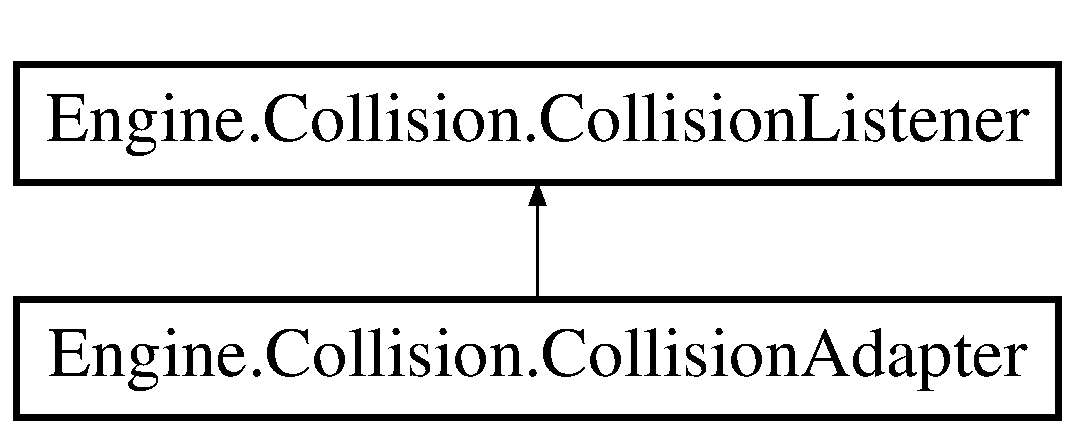
\includegraphics[height=2.000000cm]{class_engine_1_1_collision_1_1_collision_adapter}
\end{center}
\end{figure}
\subsection*{Public Member Functions}
\begin{DoxyCompactItemize}
\item 
void {\bf collisionOccurred} ({\bf CollisionEvent} e)
\end{DoxyCompactItemize}
\subsection*{Static Package Attributes}
\begin{DoxyCompactItemize}
\item 
static boolean {\bfseries ru} = true\label{class_engine_1_1_collision_1_1_collision_adapter_a7fb96009605a7a75dd321ffc051a8e10}

\end{DoxyCompactItemize}


\subsection{Detailed Description}
Created by IntelliJ IDEA. User: Sina Date: 10/26/11 Time: 2:40 PM To change this template use File $|$ Settings $|$ File Templates. 

\subsection{Member Function Documentation}
\index{Engine::Collision::CollisionAdapter@{Engine::Collision::CollisionAdapter}!collisionOccurred@{collisionOccurred}}
\index{collisionOccurred@{collisionOccurred}!Engine::Collision::CollisionAdapter@{Engine::Collision::CollisionAdapter}}
\subsubsection[{collisionOccurred}]{\setlength{\rightskip}{0pt plus 5cm}void Engine.Collision.CollisionAdapter.collisionOccurred (
\begin{DoxyParamCaption}
\item[{{\bf CollisionEvent}}]{ e}
\end{DoxyParamCaption}
)}\label{class_engine_1_1_collision_1_1_collision_adapter_a7e8127d3f0793f74093f0bfa6d2156dc}
handles the collision event based on different types of objects


\begin{DoxyParams}{Parameters}
\item[{\em e}]fired collision event from the world class \end{DoxyParams}


Implements {\bf Engine.Collision.CollisionListener} \doxyref{}{p.}{interface_engine_1_1_collision_1_1_collision_listener}.



The documentation for this class was generated from the following file:\begin{DoxyCompactItemize}
\item 
src/Engine/Collision/CollisionAdapter.java\end{DoxyCompactItemize}

\section{Engine.Collision.CollisionEvent Class Reference}
\label{class_engine_1_1_collision_1_1_collision_event}\index{Engine::Collision::CollisionEvent@{Engine::Collision::CollisionEvent}}


Inherits java::util::EventObject.

\subsection*{Public Member Functions}
\begin{DoxyCompactItemize}
\item 
{\bf CollisionEvent} ({\bf Object2D} source, {\bf Object2D} other, {\bf Vector2D} translation, boolean intersected, boolean willIntersect)
\item 
{\bf CollisionEvent} ({\bf Object2D} source)
\item 
{\bf Object2D} {\bf getOther} ()
\item 
void {\bf setOther} ({\bf Object2D} other)
\item 
{\bf Vector2D} {\bf getTranslation} ()
\item 
void {\bf setTranslation} ({\bf Vector2D} translation)
\item 
boolean {\bf isIntersected} ()
\item 
void {\bf setIntersected} (boolean intersected)
\item 
boolean {\bf isWillIntersect} ()
\item 
void {\bf setWillIntersect} (boolean willIntersect)
\end{DoxyCompactItemize}
\subsection*{Package Attributes}
\begin{DoxyCompactItemize}
\item 
{\bf Object2D} {\bfseries other}\label{class_engine_1_1_collision_1_1_collision_event_adf789749e2947ab1217b15e4ceff1229}

\item 
{\bf Vector2D} {\bfseries translation}\label{class_engine_1_1_collision_1_1_collision_event_acf8007af2bc4791d649b92f365e76367}

\item 
boolean {\bfseries intersected}\label{class_engine_1_1_collision_1_1_collision_event_a7de3da3f4b28d158ec1e7acd7a75a2f6}

\item 
boolean {\bfseries willIntersect}\label{class_engine_1_1_collision_1_1_collision_event_a49433d2223f28f82c79da1c4fd2dd7f9}

\end{DoxyCompactItemize}


\subsection{Detailed Description}
Created by IntelliJ IDEA. User: Sina Solaimanpour Date: 10/18/11 Time: 10:36 PM 

\subsection{Constructor \& Destructor Documentation}
\index{Engine::Collision::CollisionEvent@{Engine::Collision::CollisionEvent}!CollisionEvent@{CollisionEvent}}
\index{CollisionEvent@{CollisionEvent}!Engine::Collision::CollisionEvent@{Engine::Collision::CollisionEvent}}
\subsubsection[{CollisionEvent}]{\setlength{\rightskip}{0pt plus 5cm}Engine.Collision.CollisionEvent.CollisionEvent (
\begin{DoxyParamCaption}
\item[{{\bf Object2D}}]{ source, }
\item[{{\bf Object2D}}]{ other, }
\item[{{\bf Vector2D}}]{ translation, }
\item[{boolean}]{ intersected, }
\item[{boolean}]{ willIntersect}
\end{DoxyParamCaption}
)}\label{class_engine_1_1_collision_1_1_collision_event_af991ba11c5a0f3e0e38eea49b24162f9}
Creates a Collision Event To Hold The Collision's Data Needed By The Handler


\begin{DoxyParams}{Parameters}
\item[{\em source}]The Source Object of The Collision \item[{\em other}]The Other Object of The Collision \item[{\em translation}]The Correction Vector For The Source Object \item[{\em intersected}]a Boolean Which Indicates if There Are Any Collision \item[{\em willIntersect}]a Boolean Which Indicated if a Collision Will Happen Later Or Not \end{DoxyParams}
\index{Engine::Collision::CollisionEvent@{Engine::Collision::CollisionEvent}!CollisionEvent@{CollisionEvent}}
\index{CollisionEvent@{CollisionEvent}!Engine::Collision::CollisionEvent@{Engine::Collision::CollisionEvent}}
\subsubsection[{CollisionEvent}]{\setlength{\rightskip}{0pt plus 5cm}Engine.Collision.CollisionEvent.CollisionEvent (
\begin{DoxyParamCaption}
\item[{{\bf Object2D}}]{ source}
\end{DoxyParamCaption}
)}\label{class_engine_1_1_collision_1_1_collision_event_a2f546d05233e127d84e61780691a3ff4}
Default Constructor For The \doxyref{CollisionEvent}{p.}{class_engine_1_1_collision_1_1_collision_event} Note: This Constructor Should Not be Used At All!!!


\begin{DoxyParams}{Parameters}
\item[{\em source}]The Source Object of The Collision \end{DoxyParams}


\subsection{Member Function Documentation}
\index{Engine::Collision::CollisionEvent@{Engine::Collision::CollisionEvent}!getOther@{getOther}}
\index{getOther@{getOther}!Engine::Collision::CollisionEvent@{Engine::Collision::CollisionEvent}}
\subsubsection[{getOther}]{\setlength{\rightskip}{0pt plus 5cm}{\bf Object2D} Engine.Collision.CollisionEvent.getOther (
\begin{DoxyParamCaption}
{}
\end{DoxyParamCaption}
)}\label{class_engine_1_1_collision_1_1_collision_event_a29c7a1b52790c5bb75b7a62f90c048aa}
\begin{DoxyReturn}{Returns}
Returns The Other Object 
\end{DoxyReturn}
\index{Engine::Collision::CollisionEvent@{Engine::Collision::CollisionEvent}!getTranslation@{getTranslation}}
\index{getTranslation@{getTranslation}!Engine::Collision::CollisionEvent@{Engine::Collision::CollisionEvent}}
\subsubsection[{getTranslation}]{\setlength{\rightskip}{0pt plus 5cm}{\bf Vector2D} Engine.Collision.CollisionEvent.getTranslation (
\begin{DoxyParamCaption}
{}
\end{DoxyParamCaption}
)}\label{class_engine_1_1_collision_1_1_collision_event_a30baa7bee9ca9612538afc0489a47732}
\begin{DoxyReturn}{Returns}
Event's Translation Vector 
\end{DoxyReturn}
\index{Engine::Collision::CollisionEvent@{Engine::Collision::CollisionEvent}!isIntersected@{isIntersected}}
\index{isIntersected@{isIntersected}!Engine::Collision::CollisionEvent@{Engine::Collision::CollisionEvent}}
\subsubsection[{isIntersected}]{\setlength{\rightskip}{0pt plus 5cm}boolean Engine.Collision.CollisionEvent.isIntersected (
\begin{DoxyParamCaption}
{}
\end{DoxyParamCaption}
)}\label{class_engine_1_1_collision_1_1_collision_event_ada456cf233f9881255b3bfbf25a1f3d3}
\begin{DoxyReturn}{Returns}
if Intersection occurred 
\end{DoxyReturn}
\index{Engine::Collision::CollisionEvent@{Engine::Collision::CollisionEvent}!isWillIntersect@{isWillIntersect}}
\index{isWillIntersect@{isWillIntersect}!Engine::Collision::CollisionEvent@{Engine::Collision::CollisionEvent}}
\subsubsection[{isWillIntersect}]{\setlength{\rightskip}{0pt plus 5cm}boolean Engine.Collision.CollisionEvent.isWillIntersect (
\begin{DoxyParamCaption}
{}
\end{DoxyParamCaption}
)}\label{class_engine_1_1_collision_1_1_collision_event_a88505fefb7e47522aac55e4fa5ac9af5}
\begin{DoxyReturn}{Returns}
Checks if there will be any Intersection 
\end{DoxyReturn}
\index{Engine::Collision::CollisionEvent@{Engine::Collision::CollisionEvent}!setIntersected@{setIntersected}}
\index{setIntersected@{setIntersected}!Engine::Collision::CollisionEvent@{Engine::Collision::CollisionEvent}}
\subsubsection[{setIntersected}]{\setlength{\rightskip}{0pt plus 5cm}void Engine.Collision.CollisionEvent.setIntersected (
\begin{DoxyParamCaption}
\item[{boolean}]{ intersected}
\end{DoxyParamCaption}
)}\label{class_engine_1_1_collision_1_1_collision_event_af0955f7826c3545d9f8468d5600b1b2e}

\begin{DoxyParams}{Parameters}
\item[{\em intersected}]Sets if There's Any Intersection \end{DoxyParams}
\index{Engine::Collision::CollisionEvent@{Engine::Collision::CollisionEvent}!setOther@{setOther}}
\index{setOther@{setOther}!Engine::Collision::CollisionEvent@{Engine::Collision::CollisionEvent}}
\subsubsection[{setOther}]{\setlength{\rightskip}{0pt plus 5cm}void Engine.Collision.CollisionEvent.setOther (
\begin{DoxyParamCaption}
\item[{{\bf Object2D}}]{ other}
\end{DoxyParamCaption}
)}\label{class_engine_1_1_collision_1_1_collision_event_a9f769d6609ae447895c22cbbe94215dd}

\begin{DoxyParams}{Parameters}
\item[{\em other}]Sets The Other Object \end{DoxyParams}
\index{Engine::Collision::CollisionEvent@{Engine::Collision::CollisionEvent}!setTranslation@{setTranslation}}
\index{setTranslation@{setTranslation}!Engine::Collision::CollisionEvent@{Engine::Collision::CollisionEvent}}
\subsubsection[{setTranslation}]{\setlength{\rightskip}{0pt plus 5cm}void Engine.Collision.CollisionEvent.setTranslation (
\begin{DoxyParamCaption}
\item[{{\bf Vector2D}}]{ translation}
\end{DoxyParamCaption}
)}\label{class_engine_1_1_collision_1_1_collision_event_a67d886f20902c363bf823a314b8731f7}

\begin{DoxyParams}{Parameters}
\item[{\em translation}]Sets The Event's Translation \end{DoxyParams}
\index{Engine::Collision::CollisionEvent@{Engine::Collision::CollisionEvent}!setWillIntersect@{setWillIntersect}}
\index{setWillIntersect@{setWillIntersect}!Engine::Collision::CollisionEvent@{Engine::Collision::CollisionEvent}}
\subsubsection[{setWillIntersect}]{\setlength{\rightskip}{0pt plus 5cm}void Engine.Collision.CollisionEvent.setWillIntersect (
\begin{DoxyParamCaption}
\item[{boolean}]{ willIntersect}
\end{DoxyParamCaption}
)}\label{class_engine_1_1_collision_1_1_collision_event_a35d431f4f50884d6d623ad2c5050d3d1}

\begin{DoxyParams}{Parameters}
\item[{\em willIntersect}]Sets if There will be any intersection at the next step \end{DoxyParams}


The documentation for this class was generated from the following file:\begin{DoxyCompactItemize}
\item 
src/Engine/Collision/CollisionEvent.java\end{DoxyCompactItemize}

\section{Engine.Collision.CollisionListener Interface Reference}
\label{interface_engine_1_1_collision_1_1_collision_listener}\index{Engine::Collision::CollisionListener@{Engine::Collision::CollisionListener}}
Inheritance diagram for Engine.Collision.CollisionListener:\begin{figure}[H]
\begin{center}
\leavevmode
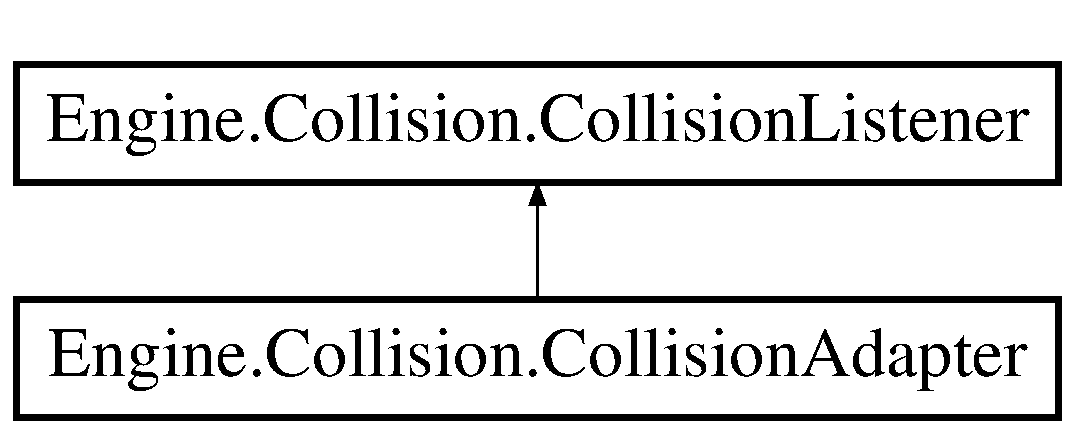
\includegraphics[height=2.000000cm]{interface_engine_1_1_collision_1_1_collision_listener}
\end{center}
\end{figure}
\subsection*{Public Member Functions}
\begin{DoxyCompactItemize}
\item 
void {\bfseries collisionOccurred} ({\bf CollisionEvent} e)\label{interface_engine_1_1_collision_1_1_collision_listener_af2ac05c2b286ac115b55930edba23f57}

\end{DoxyCompactItemize}


\subsection{Detailed Description}
Created by IntelliJ IDEA. User: Sina Solaimanpour Date: 10/18/11 Time: 10:36 PM 

The documentation for this interface was generated from the following file:\begin{DoxyCompactItemize}
\item 
src/Engine/Collision/CollisionListener.java\end{DoxyCompactItemize}

\section{Engine.EngineStarter Class Reference}
\label{class_engine_1_1_engine_starter}\index{Engine::EngineStarter@{Engine::EngineStarter}}
\subsection*{Classes}
\begin{DoxyCompactItemize}
\item 
class {\bfseries UpdateWorld}
\end{DoxyCompactItemize}
\subsection*{Public Member Functions}
\begin{DoxyCompactItemize}
\item 
{\bf EngineStarter} ({\bf World} world)
\item 
void {\bf start} ()
\item 
int {\bf getInitialDelay} ()
\item 
void {\bf setInitialDelay} (int initialDelay)
\end{DoxyCompactItemize}
\subsection*{Public Attributes}
\begin{DoxyCompactItemize}
\item 
{\bf World} {\bfseries world}\label{class_engine_1_1_engine_starter_ade1dff2ec07aad7e98ee09e39b433d72}

\end{DoxyCompactItemize}
\subsection*{Package Attributes}
\begin{DoxyCompactItemize}
\item 
int {\bfseries initialDelay} = 1000\label{class_engine_1_1_engine_starter_a28cf877a6c94d7c0c63478e80b080960}

\end{DoxyCompactItemize}


\subsection{Detailed Description}
Created by IntelliJ IDEA. User: Sina Solaimanpour Date: 10/20/11 Time: 12:09 AM 

\subsection{Constructor \& Destructor Documentation}
\index{Engine::EngineStarter@{Engine::EngineStarter}!EngineStarter@{EngineStarter}}
\index{EngineStarter@{EngineStarter}!Engine::EngineStarter@{Engine::EngineStarter}}
\subsubsection[{EngineStarter}]{\setlength{\rightskip}{0pt plus 5cm}Engine.EngineStarter.EngineStarter (
\begin{DoxyParamCaption}
\item[{{\bf World}}]{ world}
\end{DoxyParamCaption}
)}\label{class_engine_1_1_engine_starter_aeea2e7ed173b84b719b2a464d8fc07f3}
This Will Create an \doxyref{EngineStarter}{p.}{class_engine_1_1_engine_starter} Object For Staring The Simulation With Help of a Timer. 
\begin{DoxyParams}{Parameters}
\item[{\em world}]The Engine's World We Want to Start The Simulation in \end{DoxyParams}


\subsection{Member Function Documentation}
\index{Engine::EngineStarter@{Engine::EngineStarter}!getInitialDelay@{getInitialDelay}}
\index{getInitialDelay@{getInitialDelay}!Engine::EngineStarter@{Engine::EngineStarter}}
\subsubsection[{getInitialDelay}]{\setlength{\rightskip}{0pt plus 5cm}int Engine.EngineStarter.getInitialDelay (
\begin{DoxyParamCaption}
{}
\end{DoxyParamCaption}
)}\label{class_engine_1_1_engine_starter_a631f6f0cb9da926adaec4db9bedfe1d5}
\begin{DoxyReturn}{Returns}
Worlds Initial Delay 
\end{DoxyReturn}
\index{Engine::EngineStarter@{Engine::EngineStarter}!setInitialDelay@{setInitialDelay}}
\index{setInitialDelay@{setInitialDelay}!Engine::EngineStarter@{Engine::EngineStarter}}
\subsubsection[{setInitialDelay}]{\setlength{\rightskip}{0pt plus 5cm}void Engine.EngineStarter.setInitialDelay (
\begin{DoxyParamCaption}
\item[{int}]{ initialDelay}
\end{DoxyParamCaption}
)}\label{class_engine_1_1_engine_starter_ae8130a6a652c7618fba47032cb58c27b}

\begin{DoxyParams}{Parameters}
\item[{\em initialDelay}]Sets The Worlds Initial Delay Before Simulation Starts \end{DoxyParams}
\index{Engine::EngineStarter@{Engine::EngineStarter}!start@{start}}
\index{start@{start}!Engine::EngineStarter@{Engine::EngineStarter}}
\subsubsection[{start}]{\setlength{\rightskip}{0pt plus 5cm}void Engine.EngineStarter.start (
\begin{DoxyParamCaption}
{}
\end{DoxyParamCaption}
)}\label{class_engine_1_1_engine_starter_aab2c87cdbe4af223c4b125366b2111e7}
This is The Engine Start Point. This Method Will Start The Whole Simulation and Handles The Timer Object and FrameRate Related Stuff. 

The documentation for this class was generated from the following file:\begin{DoxyCompactItemize}
\item 
src/Engine/EngineStarter.java\end{DoxyCompactItemize}

\section{Engine.Forces.Force Class Reference}
\label{class_engine_1_1_forces_1_1_force}\index{Engine::Forces::Force@{Engine::Forces::Force}}
Inheritance diagram for Engine.Forces.Force:\begin{figure}[H]
\begin{center}
\leavevmode
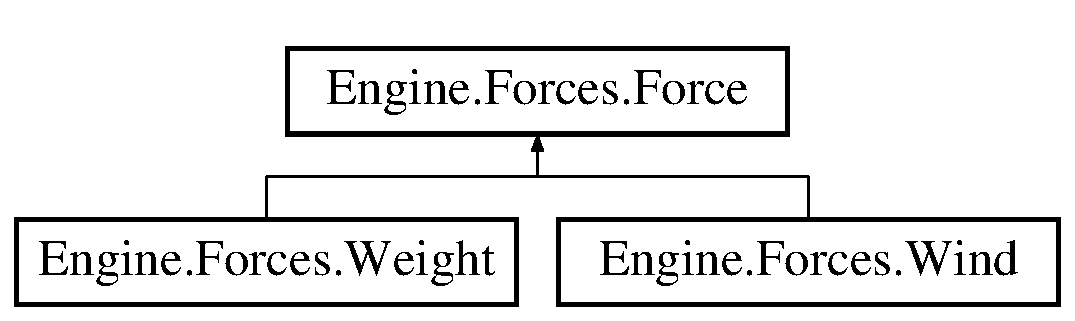
\includegraphics[height=2.000000cm]{class_engine_1_1_forces_1_1_force}
\end{center}
\end{figure}
\subsection*{Public Member Functions}
\begin{DoxyCompactItemize}
\item 
double {\bf getForceX} ()
\item 
void {\bf setForceX} (double forceX)
\item 
double {\bf getForceY} ()
\item 
void {\bf setForceY} (double forceY)
\end{DoxyCompactItemize}
\subsection*{Package Attributes}
\begin{DoxyCompactItemize}
\item 
double {\bfseries forceX}\label{class_engine_1_1_forces_1_1_force_ac5a27542e660d8c192a207bd9def4434}

\item 
double {\bfseries forceY}\label{class_engine_1_1_forces_1_1_force_a9b070b187e9fd27af9c9621cffc0125c}

\end{DoxyCompactItemize}


\subsection{Detailed Description}
Created by IntelliJ IDEA. User: Sina Solaimanpour Date: 10/18/11 Time: 10:35 PM 

\subsection{Member Function Documentation}
\index{Engine::Forces::Force@{Engine::Forces::Force}!getForceX@{getForceX}}
\index{getForceX@{getForceX}!Engine::Forces::Force@{Engine::Forces::Force}}
\subsubsection[{getForceX}]{\setlength{\rightskip}{0pt plus 5cm}double Engine.Forces.Force.getForceX (
\begin{DoxyParamCaption}
{}
\end{DoxyParamCaption}
)}\label{class_engine_1_1_forces_1_1_force_a992d0304e403ef5f64c75d00265a9396}
\begin{DoxyReturn}{Returns}
Returns \doxyref{Force}{p.}{class_engine_1_1_forces_1_1_force} Value on X Axis 
\end{DoxyReturn}
\index{Engine::Forces::Force@{Engine::Forces::Force}!getForceY@{getForceY}}
\index{getForceY@{getForceY}!Engine::Forces::Force@{Engine::Forces::Force}}
\subsubsection[{getForceY}]{\setlength{\rightskip}{0pt plus 5cm}double Engine.Forces.Force.getForceY (
\begin{DoxyParamCaption}
{}
\end{DoxyParamCaption}
)}\label{class_engine_1_1_forces_1_1_force_a83ffde6534ac328c9d708c7736c0524f}
\begin{DoxyReturn}{Returns}
Returns \doxyref{Force}{p.}{class_engine_1_1_forces_1_1_force} Value on Y Axis 
\end{DoxyReturn}
\index{Engine::Forces::Force@{Engine::Forces::Force}!setForceX@{setForceX}}
\index{setForceX@{setForceX}!Engine::Forces::Force@{Engine::Forces::Force}}
\subsubsection[{setForceX}]{\setlength{\rightskip}{0pt plus 5cm}void Engine.Forces.Force.setForceX (
\begin{DoxyParamCaption}
\item[{double}]{ forceX}
\end{DoxyParamCaption}
)}\label{class_engine_1_1_forces_1_1_force_a2738ad17b43879907d800a7cd21c1a13}

\begin{DoxyParams}{Parameters}
\item[{\em forceX}]Set The \doxyref{Force}{p.}{class_engine_1_1_forces_1_1_force} Value on X Axis \end{DoxyParams}
\index{Engine::Forces::Force@{Engine::Forces::Force}!setForceY@{setForceY}}
\index{setForceY@{setForceY}!Engine::Forces::Force@{Engine::Forces::Force}}
\subsubsection[{setForceY}]{\setlength{\rightskip}{0pt plus 5cm}void Engine.Forces.Force.setForceY (
\begin{DoxyParamCaption}
\item[{double}]{ forceY}
\end{DoxyParamCaption}
)}\label{class_engine_1_1_forces_1_1_force_a5905b1085945a92bbe07f45a834e0917}

\begin{DoxyParams}{Parameters}
\item[{\em forceX}]Set The \doxyref{Force}{p.}{class_engine_1_1_forces_1_1_force} Value on Y Axis \end{DoxyParams}


The documentation for this class was generated from the following file:\begin{DoxyCompactItemize}
\item 
src/Engine/Forces/Force.java\end{DoxyCompactItemize}

\section{Test.IterationOneTestApplication Class Reference}
\label{class_test_1_1_iteration_one_test_application}\index{Test::IterationOneTestApplication@{Test::IterationOneTestApplication}}
\subsection*{Classes}
\begin{DoxyCompactItemize}
\item 
class {\bfseries MainClass}
\end{DoxyCompactItemize}
\subsection*{Static Public Member Functions}
\begin{DoxyCompactItemize}
\item 
static void {\bfseries main} (String[$\,$] args)\label{class_test_1_1_iteration_one_test_application_a2439a7a79c575a07b8bd8bde92c2cfaf}

\end{DoxyCompactItemize}


\subsection{Detailed Description}
Created by IntelliJ IDEA. User: Sina Date: 10/31/11 Time: 11:15 AM To change this template use File $|$ Settings $|$ File Templates. 

The documentation for this class was generated from the following file:\begin{DoxyCompactItemize}
\item 
src/Test/IterationOneTestApplication.java\end{DoxyCompactItemize}

\section{Engine.Utilities.Line2D Class Reference}
\label{class_engine_1_1_utilities_1_1_line2_d}\index{Engine::Utilities::Line2D@{Engine::Utilities::Line2D}}
\subsection*{Public Member Functions}
\begin{DoxyCompactItemize}
\item 
{\bf Line2D} ({\bf Point2D} start, {\bf Point2D} end)
\item 
double {\bf getDistanceFrom} ({\bf Point2D} point)
\item 
double {\bf getParallelLineDistance} ({\bf Line2D} line)
\item 
{\bf Point2D} {\bf getStart} ()
\item 
boolean {\bf isIfInfiniteM} ()
\item 
{\bf Point2D} {\bf getEnd} ()
\item 
double {\bf getM} ()
\item 
double {\bf getC} ()
\end{DoxyCompactItemize}
\subsection*{Static Public Member Functions}
\begin{DoxyCompactItemize}
\item 
static {\bf Point2D} {\bf intersectPoint} ({\bf Line2D} line1, {\bf Line2D} line2)
\end{DoxyCompactItemize}
\subsection*{Package Attributes}
\begin{DoxyCompactItemize}
\item 
{\bf Point2D} {\bfseries start} = null\label{class_engine_1_1_utilities_1_1_line2_d_a410be554a2596b41ee02c4676a863547}

\item 
{\bf Point2D} {\bfseries end} = null\label{class_engine_1_1_utilities_1_1_line2_d_a1c053dc369de723e0a647e871887423d}

\item 
double {\bfseries m}\label{class_engine_1_1_utilities_1_1_line2_d_a5a16ff0903c1c4d27028e8b97f15353f}

\item 
double {\bfseries c}\label{class_engine_1_1_utilities_1_1_line2_d_a42304f57991970c6937cdd9643b67dd4}

\item 
boolean {\bfseries ifInfiniteM} = false\label{class_engine_1_1_utilities_1_1_line2_d_aa1cf87f0644cca088d7414e0aba3f33b}

\end{DoxyCompactItemize}


\subsection{Detailed Description}
Created by IntelliJ IDEA. User: Sina Date: 10/24/11 Time: 10:04 AM To change this template use File $|$ Settings $|$ File Templates. 

\subsection{Constructor \& Destructor Documentation}
\index{Engine::Utilities::Line2D@{Engine::Utilities::Line2D}!Line2D@{Line2D}}
\index{Line2D@{Line2D}!Engine::Utilities::Line2D@{Engine::Utilities::Line2D}}
\subsubsection[{Line2D}]{\setlength{\rightskip}{0pt plus 5cm}Engine.Utilities.Line2D.Line2D (
\begin{DoxyParamCaption}
\item[{{\bf Point2D}}]{ start, }
\item[{{\bf Point2D}}]{ end}
\end{DoxyParamCaption}
)}\label{class_engine_1_1_utilities_1_1_line2_d_a2e32c95d24e8a1b2f948f9cef4aaa3e0}
Constructor For Creating a New Line out of two Points


\begin{DoxyParams}{Parameters}
\item[{\em start}]First Point For Creating The Line \item[{\em end}]Second Point For Creating The Line \end{DoxyParams}


\subsection{Member Function Documentation}
\index{Engine::Utilities::Line2D@{Engine::Utilities::Line2D}!getC@{getC}}
\index{getC@{getC}!Engine::Utilities::Line2D@{Engine::Utilities::Line2D}}
\subsubsection[{getC}]{\setlength{\rightskip}{0pt plus 5cm}double Engine.Utilities.Line2D.getC (
\begin{DoxyParamCaption}
{}
\end{DoxyParamCaption}
)}\label{class_engine_1_1_utilities_1_1_line2_d_ade75d972cc850746b0b53d9f2c6b43b8}
\begin{DoxyReturn}{Returns}
Line's Intercept 
\end{DoxyReturn}
\index{Engine::Utilities::Line2D@{Engine::Utilities::Line2D}!getDistanceFrom@{getDistanceFrom}}
\index{getDistanceFrom@{getDistanceFrom}!Engine::Utilities::Line2D@{Engine::Utilities::Line2D}}
\subsubsection[{getDistanceFrom}]{\setlength{\rightskip}{0pt plus 5cm}double Engine.Utilities.Line2D.getDistanceFrom (
\begin{DoxyParamCaption}
\item[{{\bf Point2D}}]{ point}
\end{DoxyParamCaption}
)}\label{class_engine_1_1_utilities_1_1_line2_d_a31a9ab89417a6c10a733f32aeb452dc3}
This Will Return Minimum Distance of a Point from the line we're calling this method for.


\begin{DoxyParams}{Parameters}
\item[{\em point}]The Point to find It's distance from the line. \end{DoxyParams}
\begin{DoxyReturn}{Returns}
Point's Distance from the line which is a Double value. 
\end{DoxyReturn}
\index{Engine::Utilities::Line2D@{Engine::Utilities::Line2D}!getEnd@{getEnd}}
\index{getEnd@{getEnd}!Engine::Utilities::Line2D@{Engine::Utilities::Line2D}}
\subsubsection[{getEnd}]{\setlength{\rightskip}{0pt plus 5cm}{\bf Point2D} Engine.Utilities.Line2D.getEnd (
\begin{DoxyParamCaption}
{}
\end{DoxyParamCaption}
)}\label{class_engine_1_1_utilities_1_1_line2_d_a876c180d48c263051dd2ad9e1cbd47a9}
\begin{DoxyReturn}{Returns}
Line's End Point 
\end{DoxyReturn}
\index{Engine::Utilities::Line2D@{Engine::Utilities::Line2D}!getM@{getM}}
\index{getM@{getM}!Engine::Utilities::Line2D@{Engine::Utilities::Line2D}}
\subsubsection[{getM}]{\setlength{\rightskip}{0pt plus 5cm}double Engine.Utilities.Line2D.getM (
\begin{DoxyParamCaption}
{}
\end{DoxyParamCaption}
)}\label{class_engine_1_1_utilities_1_1_line2_d_aa8603ed53b36824cff399817e96e47da}
\begin{DoxyReturn}{Returns}
Line's tilt 
\end{DoxyReturn}
\index{Engine::Utilities::Line2D@{Engine::Utilities::Line2D}!getParallelLineDistance@{getParallelLineDistance}}
\index{getParallelLineDistance@{getParallelLineDistance}!Engine::Utilities::Line2D@{Engine::Utilities::Line2D}}
\subsubsection[{getParallelLineDistance}]{\setlength{\rightskip}{0pt plus 5cm}double Engine.Utilities.Line2D.getParallelLineDistance (
\begin{DoxyParamCaption}
\item[{{\bf Line2D}}]{ line}
\end{DoxyParamCaption}
)}\label{class_engine_1_1_utilities_1_1_line2_d_a36f5390b53454a7e1784f7109e6f9402}
Finds a line distance from the line we're calling this method for. Note: Both Lines Must Be Parallels


\begin{DoxyParams}{Parameters}
\item[{\em line}]The Line For Calculating Distance \end{DoxyParams}
\begin{DoxyReturn}{Returns}
The Distance of two Lines Which is a Double Value 
\end{DoxyReturn}
\index{Engine::Utilities::Line2D@{Engine::Utilities::Line2D}!getStart@{getStart}}
\index{getStart@{getStart}!Engine::Utilities::Line2D@{Engine::Utilities::Line2D}}
\subsubsection[{getStart}]{\setlength{\rightskip}{0pt plus 5cm}{\bf Point2D} Engine.Utilities.Line2D.getStart (
\begin{DoxyParamCaption}
{}
\end{DoxyParamCaption}
)}\label{class_engine_1_1_utilities_1_1_line2_d_a3a88c9c634e231137bd2b5eda85b1fbb}
\begin{DoxyReturn}{Returns}
Line's Start Point 
\end{DoxyReturn}
\index{Engine::Utilities::Line2D@{Engine::Utilities::Line2D}!intersectPoint@{intersectPoint}}
\index{intersectPoint@{intersectPoint}!Engine::Utilities::Line2D@{Engine::Utilities::Line2D}}
\subsubsection[{intersectPoint}]{\setlength{\rightskip}{0pt plus 5cm}static {\bf Point2D} Engine.Utilities.Line2D.intersectPoint (
\begin{DoxyParamCaption}
\item[{{\bf Line2D}}]{ line1, }
\item[{{\bf Line2D}}]{ line2}
\end{DoxyParamCaption}
)\hspace{0.3cm}{\ttfamily  [static]}}\label{class_engine_1_1_utilities_1_1_line2_d_a3840c249fc3a8a01b9d7493d87362554}
This Will find the intersecting point of two crossing lines


\begin{DoxyParams}{Parameters}
\item[{\em line1}]First Line \item[{\em line2}]Second Line \end{DoxyParams}
\begin{DoxyReturn}{Returns}
Intersecting Point of the Two Lines 
\end{DoxyReturn}
\index{Engine::Utilities::Line2D@{Engine::Utilities::Line2D}!isIfInfiniteM@{isIfInfiniteM}}
\index{isIfInfiniteM@{isIfInfiniteM}!Engine::Utilities::Line2D@{Engine::Utilities::Line2D}}
\subsubsection[{isIfInfiniteM}]{\setlength{\rightskip}{0pt plus 5cm}boolean Engine.Utilities.Line2D.isIfInfiniteM (
\begin{DoxyParamCaption}
{}
\end{DoxyParamCaption}
)}\label{class_engine_1_1_utilities_1_1_line2_d_aee6dc27e419f081bf8fb21be508824b6}
This Method Checks if the Line has an infinite tilt

\begin{DoxyReturn}{Returns}
Returns a boolean that indicates if the line has infinite tilt or not. 
\end{DoxyReturn}


The documentation for this class was generated from the following file:\begin{DoxyCompactItemize}
\item 
src/Engine/Utilities/Line2D.java\end{DoxyCompactItemize}

\section{Engine.Objects.Object2D Class Reference}
\label{class_engine_1_1_objects_1_1_object2_d}\index{Engine::Objects::Object2D@{Engine::Objects::Object2D}}
Inheritance diagram for Engine.Objects.Object2D:\begin{figure}[H]
\begin{center}
\leavevmode
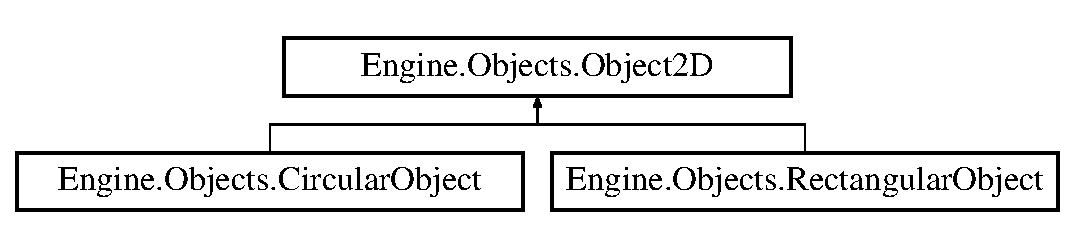
\includegraphics[height=2.000000cm]{class_engine_1_1_objects_1_1_object2_d}
\end{center}
\end{figure}
\subsection*{Public Member Functions}
\begin{DoxyCompactItemize}
\item 
{\bf Object2D} ()
\item 
void {\bf addForce} ({\bf Force} force)
\item 
void {\bf setMass} (double mass)
\item 
void {\bf setVelocity} ({\bf Velocity} velocity)
\item 
{\bf Point2D} {\bf getLocation} ()
\item 
void {\bf setLocation} ({\bf Point2D} location)
\item 
{\bf Point2D} {\bf getRotationCenter} ()
\item 
void {\bf setRotationCenter} ({\bf Point2D} rotationCenter)
\item 
void {\bf setForces} (List$<$ {\bf Force} $>$ forces)
\item 
void {\bf setFi} (double fi)
\item 
double {\bf getMass} ()
\item 
List$<$ {\bf Force} $>$ {\bf getForces} ()
\item 
{\bf Velocity} {\bf getVelocity} ()
\item 
double {\bf getFi} ()
\item 
double {\bf getAngularSpeed} ()
\item 
void {\bf setAngularSpeed} (double angularSpeed)
\end{DoxyCompactItemize}
\subsection*{Protected Member Functions}
\begin{DoxyCompactItemize}
\item 
{\bf Object2D} (double mass, {\bf Point2D} location, double fi, {\bf Velocity} velocity)
\end{DoxyCompactItemize}
\subsection*{Package Attributes}
\begin{DoxyCompactItemize}
\item 
double {\bfseries mass} = 10\label{class_engine_1_1_objects_1_1_object2_d_a27bb323298a294c1300b418f1594a035}

\item 
{\bf Point2D} {\bfseries location} = new {\bf Point2D}(10, 10)\label{class_engine_1_1_objects_1_1_object2_d_a18f9039db61d46c7a6e4eff2f9313b7b}

\item 
List$<$ {\bf Force} $>$ {\bfseries forces} = new ArrayList$<${\bf Force}$>$()\label{class_engine_1_1_objects_1_1_object2_d_a99c5e5991902d96ed7175a1b7b73cc39}

\item 
{\bf Velocity} {\bfseries velocity} = new {\bf Velocity}()\label{class_engine_1_1_objects_1_1_object2_d_af930cf1ed480768e0761ab611d124a7b}

\item 
double {\bfseries fi} = 0\label{class_engine_1_1_objects_1_1_object2_d_ad1963c50e96ce6fb67ecd4134421826c}

\item 
{\bf Point2D} {\bfseries rotationCenter} = new {\bf Point2D}(0, 0)\label{class_engine_1_1_objects_1_1_object2_d_ad9a655b0e58e7f5596285bd05633b7de}

\item 
double {\bfseries angularSpeed} = 0\label{class_engine_1_1_objects_1_1_object2_d_afa77acd6cba8ba5e559a174b79926a3b}

\end{DoxyCompactItemize}


\subsection{Detailed Description}
Created by IntelliJ IDEA. User: Sina Solaimanpour Date: 10/18/11 Time: 10:34 PM 

\subsection{Constructor \& Destructor Documentation}
\index{Engine::Objects::Object2D@{Engine::Objects::Object2D}!Object2D@{Object2D}}
\index{Object2D@{Object2D}!Engine::Objects::Object2D@{Engine::Objects::Object2D}}
\subsubsection[{Object2D}]{\setlength{\rightskip}{0pt plus 5cm}Engine.Objects.Object2D.Object2D (
\begin{DoxyParamCaption}
{}
\end{DoxyParamCaption}
)}\label{class_engine_1_1_objects_1_1_object2_d_ad8ad5818609214fb493f1ecaad3e421e}
Default Constructor For \doxyref{Object2D}{p.}{class_engine_1_1_objects_1_1_object2_d} This Will set the values as below mass = 10 location = (10,10) velocity = (0,0) fi = 0 degrees rotationCenter = (0,0) \index{Engine::Objects::Object2D@{Engine::Objects::Object2D}!Object2D@{Object2D}}
\index{Object2D@{Object2D}!Engine::Objects::Object2D@{Engine::Objects::Object2D}}
\subsubsection[{Object2D}]{\setlength{\rightskip}{0pt plus 5cm}Engine.Objects.Object2D.Object2D (
\begin{DoxyParamCaption}
\item[{double}]{ mass, }
\item[{{\bf Point2D}}]{ location, }
\item[{double}]{ fi, }
\item[{{\bf Velocity}}]{ velocity}
\end{DoxyParamCaption}
)\hspace{0.3cm}{\ttfamily  [protected]}}\label{class_engine_1_1_objects_1_1_object2_d_a83eada6c84a4613600d1cbf2c120f8a6}
Main Constructor for \doxyref{Object2D}{p.}{class_engine_1_1_objects_1_1_object2_d} Class. Notes: \doxyref{Object2D}{p.}{class_engine_1_1_objects_1_1_object2_d} is an abstract class extended by Rectangular And Circular Objects, This Constructor is used within Those Classes Constructor...


\begin{DoxyParams}{Parameters}
\item[{\em mass}]Object's Mass Value \item[{\em location}]Object's Location \item[{\em fi}]Object's rotation angle \item[{\em velocity}]Object's Velocity \end{DoxyParams}


\subsection{Member Function Documentation}
\index{Engine::Objects::Object2D@{Engine::Objects::Object2D}!addForce@{addForce}}
\index{addForce@{addForce}!Engine::Objects::Object2D@{Engine::Objects::Object2D}}
\subsubsection[{addForce}]{\setlength{\rightskip}{0pt plus 5cm}void Engine.Objects.Object2D.addForce (
\begin{DoxyParamCaption}
\item[{{\bf Force}}]{ force}
\end{DoxyParamCaption}
)}\label{class_engine_1_1_objects_1_1_object2_d_a359eb311348fd3ff4d2807955dd50eec}
This will add a new force to the forces applied to the object


\begin{DoxyParams}{Parameters}
\item[{\em force}]Force Vector \end{DoxyParams}
\index{Engine::Objects::Object2D@{Engine::Objects::Object2D}!getAngularSpeed@{getAngularSpeed}}
\index{getAngularSpeed@{getAngularSpeed}!Engine::Objects::Object2D@{Engine::Objects::Object2D}}
\subsubsection[{getAngularSpeed}]{\setlength{\rightskip}{0pt plus 5cm}double Engine.Objects.Object2D.getAngularSpeed (
\begin{DoxyParamCaption}
{}
\end{DoxyParamCaption}
)}\label{class_engine_1_1_objects_1_1_object2_d_ad8c0acc8f45d0db99f8b0b5fce1946e8}
\begin{DoxyReturn}{Returns}
Object's Angular Speed 
\end{DoxyReturn}
\index{Engine::Objects::Object2D@{Engine::Objects::Object2D}!getFi@{getFi}}
\index{getFi@{getFi}!Engine::Objects::Object2D@{Engine::Objects::Object2D}}
\subsubsection[{getFi}]{\setlength{\rightskip}{0pt plus 5cm}double Engine.Objects.Object2D.getFi (
\begin{DoxyParamCaption}
{}
\end{DoxyParamCaption}
)}\label{class_engine_1_1_objects_1_1_object2_d_aaeff1c88aba579535f81cb55d1b53bc0}
\begin{DoxyReturn}{Returns}
Object's Rotation Degree 
\end{DoxyReturn}
\index{Engine::Objects::Object2D@{Engine::Objects::Object2D}!getForces@{getForces}}
\index{getForces@{getForces}!Engine::Objects::Object2D@{Engine::Objects::Object2D}}
\subsubsection[{getForces}]{\setlength{\rightskip}{0pt plus 5cm}List$<${\bf Force}$>$ Engine.Objects.Object2D.getForces (
\begin{DoxyParamCaption}
{}
\end{DoxyParamCaption}
)}\label{class_engine_1_1_objects_1_1_object2_d_aa37f37993096f2a2203067030cb67cf9}
\begin{DoxyReturn}{Returns}
Object's Forces List 
\end{DoxyReturn}
\index{Engine::Objects::Object2D@{Engine::Objects::Object2D}!getLocation@{getLocation}}
\index{getLocation@{getLocation}!Engine::Objects::Object2D@{Engine::Objects::Object2D}}
\subsubsection[{getLocation}]{\setlength{\rightskip}{0pt plus 5cm}{\bf Point2D} Engine.Objects.Object2D.getLocation (
\begin{DoxyParamCaption}
{}
\end{DoxyParamCaption}
)}\label{class_engine_1_1_objects_1_1_object2_d_aef4d15da78d2c48e4898e782de063722}
\begin{DoxyReturn}{Returns}
Object's Location Point Without Rotation Applied 
\end{DoxyReturn}
\index{Engine::Objects::Object2D@{Engine::Objects::Object2D}!getMass@{getMass}}
\index{getMass@{getMass}!Engine::Objects::Object2D@{Engine::Objects::Object2D}}
\subsubsection[{getMass}]{\setlength{\rightskip}{0pt plus 5cm}double Engine.Objects.Object2D.getMass (
\begin{DoxyParamCaption}
{}
\end{DoxyParamCaption}
)}\label{class_engine_1_1_objects_1_1_object2_d_a507dd570ed5af46e29a7d1d3af1956c9}
\begin{DoxyReturn}{Returns}
Object's Mass 
\end{DoxyReturn}
\index{Engine::Objects::Object2D@{Engine::Objects::Object2D}!getRotationCenter@{getRotationCenter}}
\index{getRotationCenter@{getRotationCenter}!Engine::Objects::Object2D@{Engine::Objects::Object2D}}
\subsubsection[{getRotationCenter}]{\setlength{\rightskip}{0pt plus 5cm}{\bf Point2D} Engine.Objects.Object2D.getRotationCenter (
\begin{DoxyParamCaption}
{}
\end{DoxyParamCaption}
)}\label{class_engine_1_1_objects_1_1_object2_d_ae69f159fce2bfde2b2f105055ba69ca2}
\begin{DoxyReturn}{Returns}
Object's Rotation Center 
\end{DoxyReturn}
\index{Engine::Objects::Object2D@{Engine::Objects::Object2D}!getVelocity@{getVelocity}}
\index{getVelocity@{getVelocity}!Engine::Objects::Object2D@{Engine::Objects::Object2D}}
\subsubsection[{getVelocity}]{\setlength{\rightskip}{0pt plus 5cm}{\bf Velocity} Engine.Objects.Object2D.getVelocity (
\begin{DoxyParamCaption}
{}
\end{DoxyParamCaption}
)}\label{class_engine_1_1_objects_1_1_object2_d_a63a16875b5d4be0e5fd4e7a271f5b690}
\begin{DoxyReturn}{Returns}
Object's Velocity Vector 
\end{DoxyReturn}
\index{Engine::Objects::Object2D@{Engine::Objects::Object2D}!setAngularSpeed@{setAngularSpeed}}
\index{setAngularSpeed@{setAngularSpeed}!Engine::Objects::Object2D@{Engine::Objects::Object2D}}
\subsubsection[{setAngularSpeed}]{\setlength{\rightskip}{0pt plus 5cm}void Engine.Objects.Object2D.setAngularSpeed (
\begin{DoxyParamCaption}
\item[{double}]{ angularSpeed}
\end{DoxyParamCaption}
)}\label{class_engine_1_1_objects_1_1_object2_d_acf334c4443a38ab5a4a5442501f1f05c}

\begin{DoxyParams}{Parameters}
\item[{\em angularSpeed}]Set Object's Angular Speed \end{DoxyParams}
\index{Engine::Objects::Object2D@{Engine::Objects::Object2D}!setFi@{setFi}}
\index{setFi@{setFi}!Engine::Objects::Object2D@{Engine::Objects::Object2D}}
\subsubsection[{setFi}]{\setlength{\rightskip}{0pt plus 5cm}void Engine.Objects.Object2D.setFi (
\begin{DoxyParamCaption}
\item[{double}]{ fi}
\end{DoxyParamCaption}
)}\label{class_engine_1_1_objects_1_1_object2_d_a1b5918e66038af929bfdca3b1bbb6db2}

\begin{DoxyParams}{Parameters}
\item[{\em fi}]This Will Set The Object's Rotation Degree \end{DoxyParams}
\index{Engine::Objects::Object2D@{Engine::Objects::Object2D}!setForces@{setForces}}
\index{setForces@{setForces}!Engine::Objects::Object2D@{Engine::Objects::Object2D}}
\subsubsection[{setForces}]{\setlength{\rightskip}{0pt plus 5cm}void Engine.Objects.Object2D.setForces (
\begin{DoxyParamCaption}
\item[{List$<$ {\bf Force} $>$}]{ forces}
\end{DoxyParamCaption}
)}\label{class_engine_1_1_objects_1_1_object2_d_a4cb3c8defdbd84ae57faa9d999a7a2ad}

\begin{DoxyParams}{Parameters}
\item[{\em forces}]This Will Set The Whole Object's Forces \end{DoxyParams}
\index{Engine::Objects::Object2D@{Engine::Objects::Object2D}!setLocation@{setLocation}}
\index{setLocation@{setLocation}!Engine::Objects::Object2D@{Engine::Objects::Object2D}}
\subsubsection[{setLocation}]{\setlength{\rightskip}{0pt plus 5cm}void Engine.Objects.Object2D.setLocation (
\begin{DoxyParamCaption}
\item[{{\bf Point2D}}]{ location}
\end{DoxyParamCaption}
)}\label{class_engine_1_1_objects_1_1_object2_d_abe460e3e3982f229413a093e0ab35dcd}

\begin{DoxyParams}{Parameters}
\item[{\em location}]Set Object's Location Point before rotation \end{DoxyParams}
\index{Engine::Objects::Object2D@{Engine::Objects::Object2D}!setMass@{setMass}}
\index{setMass@{setMass}!Engine::Objects::Object2D@{Engine::Objects::Object2D}}
\subsubsection[{setMass}]{\setlength{\rightskip}{0pt plus 5cm}void Engine.Objects.Object2D.setMass (
\begin{DoxyParamCaption}
\item[{double}]{ mass}
\end{DoxyParamCaption}
)}\label{class_engine_1_1_objects_1_1_object2_d_a652e9f67731c97967c668c0094e6c2c2}

\begin{DoxyParams}{Parameters}
\item[{\em mass}]Returns Object's Mass \end{DoxyParams}
\index{Engine::Objects::Object2D@{Engine::Objects::Object2D}!setRotationCenter@{setRotationCenter}}
\index{setRotationCenter@{setRotationCenter}!Engine::Objects::Object2D@{Engine::Objects::Object2D}}
\subsubsection[{setRotationCenter}]{\setlength{\rightskip}{0pt plus 5cm}void Engine.Objects.Object2D.setRotationCenter (
\begin{DoxyParamCaption}
\item[{{\bf Point2D}}]{ rotationCenter}
\end{DoxyParamCaption}
)}\label{class_engine_1_1_objects_1_1_object2_d_a9465206d386ed973d623ae940314956c}

\begin{DoxyParams}{Parameters}
\item[{\em rotationCenter}]The Point Which The Object Rotates Around \end{DoxyParams}
\index{Engine::Objects::Object2D@{Engine::Objects::Object2D}!setVelocity@{setVelocity}}
\index{setVelocity@{setVelocity}!Engine::Objects::Object2D@{Engine::Objects::Object2D}}
\subsubsection[{setVelocity}]{\setlength{\rightskip}{0pt plus 5cm}void Engine.Objects.Object2D.setVelocity (
\begin{DoxyParamCaption}
\item[{{\bf Velocity}}]{ velocity}
\end{DoxyParamCaption}
)}\label{class_engine_1_1_objects_1_1_object2_d_a7df0d3b59d2b5caed31637113c59de6f}

\begin{DoxyParams}{Parameters}
\item[{\em velocity}]Object's Velocity's Vector \end{DoxyParams}


The documentation for this class was generated from the following file:\begin{DoxyCompactItemize}
\item 
src/Engine/Objects/Object2D.java\end{DoxyCompactItemize}

\section{Engine.Utilities.Point2D Class Reference}
\label{class_engine_1_1_utilities_1_1_point2_d}\index{Engine::Utilities::Point2D@{Engine::Utilities::Point2D}}
\subsection*{Public Member Functions}
\begin{DoxyCompactItemize}
\item 
{\bf Point2D} (int posX, int posY)
\item 
int {\bf getPosX} ()
\item 
void {\bf setPosX} (int posX)
\item 
int {\bf getPosY} ()
\item 
void {\bf setPosY} (int posY)
\end{DoxyCompactItemize}
\subsection*{Static Public Member Functions}
\begin{DoxyCompactItemize}
\item 
static double {\bf twoPointDistance} ({\bf Point2D} a, {\bf Point2D} b)
\end{DoxyCompactItemize}
\subsection*{Package Attributes}
\begin{DoxyCompactItemize}
\item 
int {\bfseries posX} = 0\label{class_engine_1_1_utilities_1_1_point2_d_af3c07c9105ec1571279c9ef09c1256a2}

\item 
int {\bfseries posY} = 0\label{class_engine_1_1_utilities_1_1_point2_d_a8edcae8aa3ff000e3b3fd02e2630b161}

\end{DoxyCompactItemize}


\subsection{Detailed Description}
Created by IntelliJ IDEA. User: Sina Date: 10/24/11 Time: 10:03 AM To change this template use File $|$ Settings $|$ File Templates. 

\subsection{Constructor \& Destructor Documentation}
\index{Engine::Utilities::Point2D@{Engine::Utilities::Point2D}!Point2D@{Point2D}}
\index{Point2D@{Point2D}!Engine::Utilities::Point2D@{Engine::Utilities::Point2D}}
\subsubsection[{Point2D}]{\setlength{\rightskip}{0pt plus 5cm}Engine.Utilities.Point2D.Point2D (
\begin{DoxyParamCaption}
\item[{int}]{ posX, }
\item[{int}]{ posY}
\end{DoxyParamCaption}
)}\label{class_engine_1_1_utilities_1_1_point2_d_acbe76cb3282b615b205f20885f0e1bb8}
Constructor To Create a \doxyref{Point2D}{p.}{class_engine_1_1_utilities_1_1_point2_d} 
\begin{DoxyParams}{Parameters}
\item[{\em posX}]Point2D's X Position \item[{\em posY}]Point2D's Y Position \end{DoxyParams}


\subsection{Member Function Documentation}
\index{Engine::Utilities::Point2D@{Engine::Utilities::Point2D}!getPosX@{getPosX}}
\index{getPosX@{getPosX}!Engine::Utilities::Point2D@{Engine::Utilities::Point2D}}
\subsubsection[{getPosX}]{\setlength{\rightskip}{0pt plus 5cm}int Engine.Utilities.Point2D.getPosX (
\begin{DoxyParamCaption}
{}
\end{DoxyParamCaption}
)}\label{class_engine_1_1_utilities_1_1_point2_d_aa2c415d59f2006ed9ce6d6c2b7931f84}
\begin{DoxyReturn}{Returns}
Point2D's X Position 
\end{DoxyReturn}
\index{Engine::Utilities::Point2D@{Engine::Utilities::Point2D}!getPosY@{getPosY}}
\index{getPosY@{getPosY}!Engine::Utilities::Point2D@{Engine::Utilities::Point2D}}
\subsubsection[{getPosY}]{\setlength{\rightskip}{0pt plus 5cm}int Engine.Utilities.Point2D.getPosY (
\begin{DoxyParamCaption}
{}
\end{DoxyParamCaption}
)}\label{class_engine_1_1_utilities_1_1_point2_d_acf2b50272c2bcbc46773b58dfdd003c8}
\begin{DoxyReturn}{Returns}
Point2D's Y Position 
\end{DoxyReturn}
\index{Engine::Utilities::Point2D@{Engine::Utilities::Point2D}!setPosX@{setPosX}}
\index{setPosX@{setPosX}!Engine::Utilities::Point2D@{Engine::Utilities::Point2D}}
\subsubsection[{setPosX}]{\setlength{\rightskip}{0pt plus 5cm}void Engine.Utilities.Point2D.setPosX (
\begin{DoxyParamCaption}
\item[{int}]{ posX}
\end{DoxyParamCaption}
)}\label{class_engine_1_1_utilities_1_1_point2_d_abe0d16a592ab97e8c90a9506780d03a6}

\begin{DoxyParams}{Parameters}
\item[{\em posX}]Sets Point2D's X Position \end{DoxyParams}
\index{Engine::Utilities::Point2D@{Engine::Utilities::Point2D}!setPosY@{setPosY}}
\index{setPosY@{setPosY}!Engine::Utilities::Point2D@{Engine::Utilities::Point2D}}
\subsubsection[{setPosY}]{\setlength{\rightskip}{0pt plus 5cm}void Engine.Utilities.Point2D.setPosY (
\begin{DoxyParamCaption}
\item[{int}]{ posY}
\end{DoxyParamCaption}
)}\label{class_engine_1_1_utilities_1_1_point2_d_a8edabc81e36b410fc72a840b41b253a8}

\begin{DoxyParams}{Parameters}
\item[{\em posY}]Sets Point2D's Y Position \end{DoxyParams}
\index{Engine::Utilities::Point2D@{Engine::Utilities::Point2D}!twoPointDistance@{twoPointDistance}}
\index{twoPointDistance@{twoPointDistance}!Engine::Utilities::Point2D@{Engine::Utilities::Point2D}}
\subsubsection[{twoPointDistance}]{\setlength{\rightskip}{0pt plus 5cm}static double Engine.Utilities.Point2D.twoPointDistance (
\begin{DoxyParamCaption}
\item[{{\bf Point2D}}]{ a, }
\item[{{\bf Point2D}}]{ b}
\end{DoxyParamCaption}
)\hspace{0.3cm}{\ttfamily  [static]}}\label{class_engine_1_1_utilities_1_1_point2_d_a2ad5742e14df78659404ea646cd1b1b1}
Calculates Distance Between two Point2Ds 
\begin{DoxyParams}{Parameters}
\item[{\em a}]The First \doxyref{Point2D}{p.}{class_engine_1_1_utilities_1_1_point2_d} \item[{\em b}]The Second \doxyref{Point2D}{p.}{class_engine_1_1_utilities_1_1_point2_d} \end{DoxyParams}
\begin{DoxyReturn}{Returns}
The Distance Between two Point2Ds 
\end{DoxyReturn}


The documentation for this class was generated from the following file:\begin{DoxyCompactItemize}
\item 
src/Engine/Utilities/Point2D.java\end{DoxyCompactItemize}

\section{Engine.Properties Interface Reference}
\label{interface_engine_1_1_properties}\index{Engine::Properties@{Engine::Properties}}
\subsection*{Static Public Attributes}
\begin{DoxyCompactItemize}
\item 
static final double {\bf timeStep} = 1 / 9
\item 
static final int {\bf engineWait} = 50
\item 
static final boolean {\bf wired} = true
\end{DoxyCompactItemize}


\subsection{Detailed Description}
Created by IntelliJ IDEA. User: Sina Solaimanpour Date: 10/20/11 Time: 3:07 AM 

\subsection{Member Data Documentation}
\index{Engine::Properties@{Engine::Properties}!engineWait@{engineWait}}
\index{engineWait@{engineWait}!Engine::Properties@{Engine::Properties}}
\subsubsection[{engineWait}]{\setlength{\rightskip}{0pt plus 5cm}final int {\bf Engine.Properties.engineWait} = 50\hspace{0.3cm}{\ttfamily  [static]}}\label{interface_engine_1_1_properties_af6d32581cbe4eddbdcb9247ca68915cc}
Engine Waits for engineWait MilliSeconds Then Render The Whole World Again \index{Engine::Properties@{Engine::Properties}!timeStep@{timeStep}}
\index{timeStep@{timeStep}!Engine::Properties@{Engine::Properties}}
\subsubsection[{timeStep}]{\setlength{\rightskip}{0pt plus 5cm}final double {\bf Engine.Properties.timeStep} = 1 / 9\hspace{0.3cm}{\ttfamily  [static]}}\label{interface_engine_1_1_properties_a7bf35fba40c4928c6cca56d0bda158fa}
Time Steps Which Acts as DeltaT in Real World's Physics Formulations \index{Engine::Properties@{Engine::Properties}!wired@{wired}}
\index{wired@{wired}!Engine::Properties@{Engine::Properties}}
\subsubsection[{wired}]{\setlength{\rightskip}{0pt plus 5cm}final boolean {\bf Engine.Properties.wired} = true\hspace{0.3cm}{\ttfamily  [static]}}\label{interface_engine_1_1_properties_a974c223ea8ba285c7ffe2a4c89e55652}
If True Then The Objects Will Be Drawn as Wired Objects if False The Objects Will Be Drawn with Filled Color 

The documentation for this interface was generated from the following file:\begin{DoxyCompactItemize}
\item 
src/Engine/Properties.java\end{DoxyCompactItemize}

\section{Engine.Objects.RectangularObject Class Reference}
\label{class_engine_1_1_objects_1_1_rectangular_object}\index{Engine::Objects::RectangularObject@{Engine::Objects::RectangularObject}}
Inheritance diagram for Engine.Objects.RectangularObject:\begin{figure}[H]
\begin{center}
\leavevmode
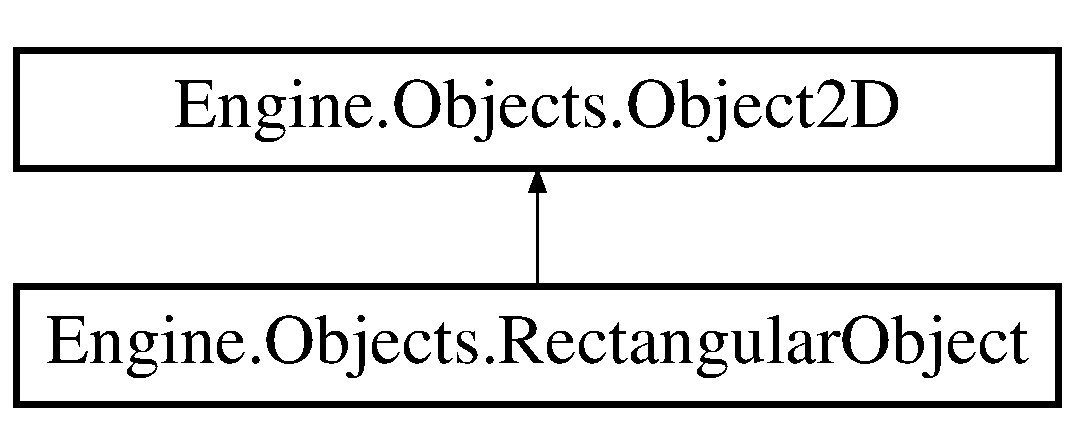
\includegraphics[height=2.000000cm]{class_engine_1_1_objects_1_1_rectangular_object}
\end{center}
\end{figure}
\subsection*{Public Member Functions}
\begin{DoxyCompactItemize}
\item 
{\bf RectangularObject} ()
\item 
{\bf RectangularObject} (int width, int length)
\item 
{\bf RectangularObject} (double mass, {\bf Point2D} location, double fi, {\bf Velocity} velocity, int width, int length)
\item 
int {\bf getWidth} ()
\item 
void {\bf setWidth} (int width)
\item 
{\bf Point2D} {\bf getUpperLeftCorner} ()
\item 
void {\bf setUpperLeftCorner} ({\bf Point2D} upperLeftCorner)
\item 
{\bf Point2D} {\bf getUpperRightCorner} ()
\item 
void {\bf setUpperRightCorner} ({\bf Point2D} upperRightCorner)
\item 
{\bf Point2D} {\bf getLowerRightCorner} ()
\item 
void {\bf setLowerRightCorner} ({\bf Point2D} lowerRightCorner)
\item 
{\bf Point2D} {\bf getLowerLeftCorner} ()
\item 
void {\bf setLowerLeftCorner} ({\bf Point2D} lowerLeftCorner)
\item 
int {\bf getLength} ()
\item 
void {\bf setLength} (int length)
\item 
List$<$ {\bf Point2D} $>$ {\bf getPoints} ()
\item 
List$<$ {\bf Vector2D} $>$ {\bf getEdges} ()
\item 
void {\bf updateEdges} ()
\item 
void {\bf updateCenter} ()
\item 
{\bf Point2D} {\bf getCenter} ()
\item 
void {\bf setCenter} ({\bf Point2D} center)
\end{DoxyCompactItemize}
\subsection*{Package Attributes}
\begin{DoxyCompactItemize}
\item 
int {\bfseries width} = 100\label{class_engine_1_1_objects_1_1_rectangular_object_a278b25b08ef46d4ae8c3d2dab4616e56}

\item 
int {\bfseries length} = 100\label{class_engine_1_1_objects_1_1_rectangular_object_a914fdabdb38f3c6bfe2cecff490d21d8}

\item 
List$<$ {\bf Point2D} $>$ {\bfseries points} = new ArrayList$<${\bf Point2D}$>$()\label{class_engine_1_1_objects_1_1_rectangular_object_a1509b26c3756567ce0045324cf8b25bd}

\item 
List$<$ {\bf Vector2D} $>$ {\bfseries edges} = new ArrayList$<${\bf Vector2D}$>$()\label{class_engine_1_1_objects_1_1_rectangular_object_aaa8177c30e2ba78601523fa709fa6a9f}

\item 
{\bf Point2D} {\bfseries center}\label{class_engine_1_1_objects_1_1_rectangular_object_ae0f8698120bd06984caf10bf4ddd7999}

\end{DoxyCompactItemize}


\subsection{Detailed Description}
Created by IntelliJ IDEA. User: Sina Solaimanpour Date: 10/18/11 Time: 10:41 PM 

\subsection{Constructor \& Destructor Documentation}
\index{Engine::Objects::RectangularObject@{Engine::Objects::RectangularObject}!RectangularObject@{RectangularObject}}
\index{RectangularObject@{RectangularObject}!Engine::Objects::RectangularObject@{Engine::Objects::RectangularObject}}
\subsubsection[{RectangularObject}]{\setlength{\rightskip}{0pt plus 5cm}Engine.Objects.RectangularObject.RectangularObject (
\begin{DoxyParamCaption}
{}
\end{DoxyParamCaption}
)}\label{class_engine_1_1_objects_1_1_rectangular_object_a9a11ce7d1789f0cdd771cb1741b66503}
Rectangular Object's Default Constructor This will set the objects properties to the default values as below: width = 100 length = 100 (All The Other Values is set as The Object2D's default amounts...) \index{Engine::Objects::RectangularObject@{Engine::Objects::RectangularObject}!RectangularObject@{RectangularObject}}
\index{RectangularObject@{RectangularObject}!Engine::Objects::RectangularObject@{Engine::Objects::RectangularObject}}
\subsubsection[{RectangularObject}]{\setlength{\rightskip}{0pt plus 5cm}Engine.Objects.RectangularObject.RectangularObject (
\begin{DoxyParamCaption}
\item[{int}]{ width, }
\item[{int}]{ length}
\end{DoxyParamCaption}
)}\label{class_engine_1_1_objects_1_1_rectangular_object_ae0a419cbf5b78c340e9c1706086ab6d3}
This constructor will get the width and length of the object and other properties will be set as default This will also sets the Object's default Rotation Center Point


\begin{DoxyParams}{Parameters}
\item[{\em width}]Object's Width \item[{\em length}]Object's Length \end{DoxyParams}
\index{Engine::Objects::RectangularObject@{Engine::Objects::RectangularObject}!RectangularObject@{RectangularObject}}
\index{RectangularObject@{RectangularObject}!Engine::Objects::RectangularObject@{Engine::Objects::RectangularObject}}
\subsubsection[{RectangularObject}]{\setlength{\rightskip}{0pt plus 5cm}Engine.Objects.RectangularObject.RectangularObject (
\begin{DoxyParamCaption}
\item[{double}]{ mass, }
\item[{{\bf Point2D}}]{ location, }
\item[{double}]{ fi, }
\item[{{\bf Velocity}}]{ velocity, }
\item[{int}]{ width, }
\item[{int}]{ length}
\end{DoxyParamCaption}
)}\label{class_engine_1_1_objects_1_1_rectangular_object_a803b5efa87ca23322b0d7f08744d6e05}
Rectangular Object's Main Constructor This will also sets the Object's default Rotation Center Point


\begin{DoxyParams}{Parameters}
\item[{\em mass}]Object's Mass \item[{\em location}]Object's Location Point \item[{\em fi}]Object's Rotation Value \item[{\em velocity}]Object's Velocity Vector \item[{\em width}]Object's Width \item[{\em length}]Object's Length \end{DoxyParams}


\subsection{Member Function Documentation}
\index{Engine::Objects::RectangularObject@{Engine::Objects::RectangularObject}!getCenter@{getCenter}}
\index{getCenter@{getCenter}!Engine::Objects::RectangularObject@{Engine::Objects::RectangularObject}}
\subsubsection[{getCenter}]{\setlength{\rightskip}{0pt plus 5cm}{\bf Point2D} Engine.Objects.RectangularObject.getCenter (
\begin{DoxyParamCaption}
{}
\end{DoxyParamCaption}
)}\label{class_engine_1_1_objects_1_1_rectangular_object_a75b4dfe5e39fc25d694c957d9f73460d}
\begin{DoxyReturn}{Returns}
Returns Object's Center point 
\end{DoxyReturn}
\index{Engine::Objects::RectangularObject@{Engine::Objects::RectangularObject}!getEdges@{getEdges}}
\index{getEdges@{getEdges}!Engine::Objects::RectangularObject@{Engine::Objects::RectangularObject}}
\subsubsection[{getEdges}]{\setlength{\rightskip}{0pt plus 5cm}List$<${\bf Vector2D}$>$ Engine.Objects.RectangularObject.getEdges (
\begin{DoxyParamCaption}
{}
\end{DoxyParamCaption}
)}\label{class_engine_1_1_objects_1_1_rectangular_object_aad67d466505cff481d0d1469b3bdb1ed}
\begin{DoxyReturn}{Returns}
It Returns Object's Edges for collision detection 
\end{DoxyReturn}
\index{Engine::Objects::RectangularObject@{Engine::Objects::RectangularObject}!getLength@{getLength}}
\index{getLength@{getLength}!Engine::Objects::RectangularObject@{Engine::Objects::RectangularObject}}
\subsubsection[{getLength}]{\setlength{\rightskip}{0pt plus 5cm}int Engine.Objects.RectangularObject.getLength (
\begin{DoxyParamCaption}
{}
\end{DoxyParamCaption}
)}\label{class_engine_1_1_objects_1_1_rectangular_object_a17a2ff9146b43d99f997ed9ab66922b9}
\begin{DoxyReturn}{Returns}
Object's Length 
\end{DoxyReturn}
\index{Engine::Objects::RectangularObject@{Engine::Objects::RectangularObject}!getLowerLeftCorner@{getLowerLeftCorner}}
\index{getLowerLeftCorner@{getLowerLeftCorner}!Engine::Objects::RectangularObject@{Engine::Objects::RectangularObject}}
\subsubsection[{getLowerLeftCorner}]{\setlength{\rightskip}{0pt plus 5cm}{\bf Point2D} Engine.Objects.RectangularObject.getLowerLeftCorner (
\begin{DoxyParamCaption}
{}
\end{DoxyParamCaption}
)}\label{class_engine_1_1_objects_1_1_rectangular_object_a5f16f6bdea5235c69a0d03df9c5ba31f}
\begin{DoxyReturn}{Returns}
Object's Lower Left Corner Point 
\end{DoxyReturn}
\index{Engine::Objects::RectangularObject@{Engine::Objects::RectangularObject}!getLowerRightCorner@{getLowerRightCorner}}
\index{getLowerRightCorner@{getLowerRightCorner}!Engine::Objects::RectangularObject@{Engine::Objects::RectangularObject}}
\subsubsection[{getLowerRightCorner}]{\setlength{\rightskip}{0pt plus 5cm}{\bf Point2D} Engine.Objects.RectangularObject.getLowerRightCorner (
\begin{DoxyParamCaption}
{}
\end{DoxyParamCaption}
)}\label{class_engine_1_1_objects_1_1_rectangular_object_aa10619ba75ac2bb723f10e40105ce85a}
\begin{DoxyReturn}{Returns}
Object's Lower Right Corner Point 
\end{DoxyReturn}
\index{Engine::Objects::RectangularObject@{Engine::Objects::RectangularObject}!getPoints@{getPoints}}
\index{getPoints@{getPoints}!Engine::Objects::RectangularObject@{Engine::Objects::RectangularObject}}
\subsubsection[{getPoints}]{\setlength{\rightskip}{0pt plus 5cm}List$<${\bf Point2D}$>$ Engine.Objects.RectangularObject.getPoints (
\begin{DoxyParamCaption}
{}
\end{DoxyParamCaption}
)}\label{class_engine_1_1_objects_1_1_rectangular_object_a71a1a1c451c590fa55e9022eaccbb5d1}
\begin{DoxyReturn}{Returns}
Object's Corners Point 
\end{DoxyReturn}
\index{Engine::Objects::RectangularObject@{Engine::Objects::RectangularObject}!getUpperLeftCorner@{getUpperLeftCorner}}
\index{getUpperLeftCorner@{getUpperLeftCorner}!Engine::Objects::RectangularObject@{Engine::Objects::RectangularObject}}
\subsubsection[{getUpperLeftCorner}]{\setlength{\rightskip}{0pt plus 5cm}{\bf Point2D} Engine.Objects.RectangularObject.getUpperLeftCorner (
\begin{DoxyParamCaption}
{}
\end{DoxyParamCaption}
)}\label{class_engine_1_1_objects_1_1_rectangular_object_a118aa33005ea06d60fffb7713aed1c5f}
\begin{DoxyReturn}{Returns}
Object's Upper Left Corner Point 
\end{DoxyReturn}
\index{Engine::Objects::RectangularObject@{Engine::Objects::RectangularObject}!getUpperRightCorner@{getUpperRightCorner}}
\index{getUpperRightCorner@{getUpperRightCorner}!Engine::Objects::RectangularObject@{Engine::Objects::RectangularObject}}
\subsubsection[{getUpperRightCorner}]{\setlength{\rightskip}{0pt plus 5cm}{\bf Point2D} Engine.Objects.RectangularObject.getUpperRightCorner (
\begin{DoxyParamCaption}
{}
\end{DoxyParamCaption}
)}\label{class_engine_1_1_objects_1_1_rectangular_object_a5143ad2915006bbfe4a5189c36872e0b}
\begin{DoxyReturn}{Returns}
Object's Upper Right Corner Point 
\end{DoxyReturn}
\index{Engine::Objects::RectangularObject@{Engine::Objects::RectangularObject}!getWidth@{getWidth}}
\index{getWidth@{getWidth}!Engine::Objects::RectangularObject@{Engine::Objects::RectangularObject}}
\subsubsection[{getWidth}]{\setlength{\rightskip}{0pt plus 5cm}int Engine.Objects.RectangularObject.getWidth (
\begin{DoxyParamCaption}
{}
\end{DoxyParamCaption}
)}\label{class_engine_1_1_objects_1_1_rectangular_object_a23fa74b223f72367440b6a141701d704}
\begin{DoxyReturn}{Returns}
Object's Width 
\end{DoxyReturn}
\index{Engine::Objects::RectangularObject@{Engine::Objects::RectangularObject}!setCenter@{setCenter}}
\index{setCenter@{setCenter}!Engine::Objects::RectangularObject@{Engine::Objects::RectangularObject}}
\subsubsection[{setCenter}]{\setlength{\rightskip}{0pt plus 5cm}void Engine.Objects.RectangularObject.setCenter (
\begin{DoxyParamCaption}
\item[{{\bf Point2D}}]{ center}
\end{DoxyParamCaption}
)}\label{class_engine_1_1_objects_1_1_rectangular_object_aa5729fb596ec8ed83e73ca96433cb192}

\begin{DoxyParams}{Parameters}
\item[{\em center}]Sets Object's Center Point \end{DoxyParams}
\index{Engine::Objects::RectangularObject@{Engine::Objects::RectangularObject}!setLength@{setLength}}
\index{setLength@{setLength}!Engine::Objects::RectangularObject@{Engine::Objects::RectangularObject}}
\subsubsection[{setLength}]{\setlength{\rightskip}{0pt plus 5cm}void Engine.Objects.RectangularObject.setLength (
\begin{DoxyParamCaption}
\item[{int}]{ length}
\end{DoxyParamCaption}
)}\label{class_engine_1_1_objects_1_1_rectangular_object_a1f02fbb68f607a7080d30e6c528d420c}

\begin{DoxyParams}{Parameters}
\item[{\em length}]Sets Object's Length and it will also sets the rotation center's X Value as length / 2 \end{DoxyParams}
\index{Engine::Objects::RectangularObject@{Engine::Objects::RectangularObject}!setLowerLeftCorner@{setLowerLeftCorner}}
\index{setLowerLeftCorner@{setLowerLeftCorner}!Engine::Objects::RectangularObject@{Engine::Objects::RectangularObject}}
\subsubsection[{setLowerLeftCorner}]{\setlength{\rightskip}{0pt plus 5cm}void Engine.Objects.RectangularObject.setLowerLeftCorner (
\begin{DoxyParamCaption}
\item[{{\bf Point2D}}]{ lowerLeftCorner}
\end{DoxyParamCaption}
)}\label{class_engine_1_1_objects_1_1_rectangular_object_a6b40fee91b4130b9f3ff5023d061da02}

\begin{DoxyParams}{Parameters}
\item[{\em lowerLeftCorner}]Sets Object's Lower Left Corner Point \end{DoxyParams}
\index{Engine::Objects::RectangularObject@{Engine::Objects::RectangularObject}!setLowerRightCorner@{setLowerRightCorner}}
\index{setLowerRightCorner@{setLowerRightCorner}!Engine::Objects::RectangularObject@{Engine::Objects::RectangularObject}}
\subsubsection[{setLowerRightCorner}]{\setlength{\rightskip}{0pt plus 5cm}void Engine.Objects.RectangularObject.setLowerRightCorner (
\begin{DoxyParamCaption}
\item[{{\bf Point2D}}]{ lowerRightCorner}
\end{DoxyParamCaption}
)}\label{class_engine_1_1_objects_1_1_rectangular_object_a8814fb6a892e57158d3c21780b024806}

\begin{DoxyParams}{Parameters}
\item[{\em lowerRightCorner}]Sets Object's Lower Right Corner Point \end{DoxyParams}
\index{Engine::Objects::RectangularObject@{Engine::Objects::RectangularObject}!setUpperLeftCorner@{setUpperLeftCorner}}
\index{setUpperLeftCorner@{setUpperLeftCorner}!Engine::Objects::RectangularObject@{Engine::Objects::RectangularObject}}
\subsubsection[{setUpperLeftCorner}]{\setlength{\rightskip}{0pt plus 5cm}void Engine.Objects.RectangularObject.setUpperLeftCorner (
\begin{DoxyParamCaption}
\item[{{\bf Point2D}}]{ upperLeftCorner}
\end{DoxyParamCaption}
)}\label{class_engine_1_1_objects_1_1_rectangular_object_a618952117dbe8a5f04709e591c7d88aa}

\begin{DoxyParams}{Parameters}
\item[{\em upperLeftCorner}]Sets Object's Upper Left Corner Point \end{DoxyParams}
\index{Engine::Objects::RectangularObject@{Engine::Objects::RectangularObject}!setUpperRightCorner@{setUpperRightCorner}}
\index{setUpperRightCorner@{setUpperRightCorner}!Engine::Objects::RectangularObject@{Engine::Objects::RectangularObject}}
\subsubsection[{setUpperRightCorner}]{\setlength{\rightskip}{0pt plus 5cm}void Engine.Objects.RectangularObject.setUpperRightCorner (
\begin{DoxyParamCaption}
\item[{{\bf Point2D}}]{ upperRightCorner}
\end{DoxyParamCaption}
)}\label{class_engine_1_1_objects_1_1_rectangular_object_a8f5cc22a68f27e202707bfc9084eff24}

\begin{DoxyParams}{Parameters}
\item[{\em upperRightCorner}]Sets Upper Corner Point \end{DoxyParams}
\index{Engine::Objects::RectangularObject@{Engine::Objects::RectangularObject}!setWidth@{setWidth}}
\index{setWidth@{setWidth}!Engine::Objects::RectangularObject@{Engine::Objects::RectangularObject}}
\subsubsection[{setWidth}]{\setlength{\rightskip}{0pt plus 5cm}void Engine.Objects.RectangularObject.setWidth (
\begin{DoxyParamCaption}
\item[{int}]{ width}
\end{DoxyParamCaption}
)}\label{class_engine_1_1_objects_1_1_rectangular_object_a3b5b94ba430b7a0fb731a0bf5fe7ed83}

\begin{DoxyParams}{Parameters}
\item[{\em width}]Sets Object's Width \end{DoxyParams}
\index{Engine::Objects::RectangularObject@{Engine::Objects::RectangularObject}!updateCenter@{updateCenter}}
\index{updateCenter@{updateCenter}!Engine::Objects::RectangularObject@{Engine::Objects::RectangularObject}}
\subsubsection[{updateCenter}]{\setlength{\rightskip}{0pt plus 5cm}void Engine.Objects.RectangularObject.updateCenter (
\begin{DoxyParamCaption}
{}
\end{DoxyParamCaption}
)}\label{class_engine_1_1_objects_1_1_rectangular_object_a2d171ff562ecd0ce6c6c0759ebe30702}
This Will Updates The object's center point based on the new Corners after Object's Rotation \index{Engine::Objects::RectangularObject@{Engine::Objects::RectangularObject}!updateEdges@{updateEdges}}
\index{updateEdges@{updateEdges}!Engine::Objects::RectangularObject@{Engine::Objects::RectangularObject}}
\subsubsection[{updateEdges}]{\setlength{\rightskip}{0pt plus 5cm}void Engine.Objects.RectangularObject.updateEdges (
\begin{DoxyParamCaption}
{}
\end{DoxyParamCaption}
)}\label{class_engine_1_1_objects_1_1_rectangular_object_a8e7dc6958d6776b4706e28091adcfa39}
This Method Will Updates the object's Edges based on the new Corners after Object's Rotation 

The documentation for this class was generated from the following file:\begin{DoxyCompactItemize}
\item 
src/Engine/Objects/RectangularObject.java\end{DoxyCompactItemize}

\section{Test.TestApp1 Class Reference}
\label{class_test_1_1_test_app1}\index{Test::TestApp1@{Test::TestApp1}}
\subsection*{Static Public Member Functions}
\begin{DoxyCompactItemize}
\item 
static void {\bfseries main} (String[$\,$] args)\label{class_test_1_1_test_app1_a1fd610da861cd5670b913e275e0b62bb}

\end{DoxyCompactItemize}


\subsection{Detailed Description}
Created by IntelliJ IDEA. User: Sina Solaimanpour Date: 10/18/11 Time: 10:48 PM 

The documentation for this class was generated from the following file:\begin{DoxyCompactItemize}
\item 
src/Test/TestApp1.java\end{DoxyCompactItemize}

\section{Engine.Utilities.Vector2D Class Reference}
\label{class_engine_1_1_utilities_1_1_vector2_d}\index{Engine::Utilities::Vector2D@{Engine::Utilities::Vector2D}}
\subsection*{Public Member Functions}
\begin{DoxyCompactItemize}
\item 
{\bf Vector2D} ()
\item 
{\bf Vector2D} (double x, double y)
\item 
double {\bf magnitude} ()
\item 
void {\bf normalize} ()
\item 
{\bf Vector2D} {\bf getNormalized} ()
\item 
double {\bf dotProduct} ({\bf Vector2D} vector)
\item 
double {\bf distanceTo} ({\bf Vector2D} vector)
\item 
boolean {\bf equals} (Object obj)
\item 
boolean {\bf equals} ({\bf Vector2D} v)
\item 
String {\bf toString} ()
\item 
double {\bf getX} ()
\item 
void {\bf setX} (double x)
\item 
double {\bf getY} ()
\item 
void {\bf setY} (double y)
\end{DoxyCompactItemize}
\subsection*{Static Public Member Functions}
\begin{DoxyCompactItemize}
\item 
static {\bf Vector2D} {\bf fromPoint} ({\bf Point2D} p)
\item 
static {\bf Vector2D} {\bf fromPoint} (int x, int y)
\item 
static {\bf Vector2D} {\bf plus} ({\bf Vector2D} a, {\bf Vector2D} b)
\item 
static {\bf Vector2D} {\bf minus} ({\bf Vector2D} a)
\item 
static {\bf Vector2D} {\bf minus} ({\bf Vector2D} a, {\bf Vector2D} b)
\item 
static {\bf Vector2D} {\bf multiply} ({\bf Vector2D} a, double b)
\item 
static {\bf Vector2D} {\bf multiply} ({\bf Vector2D} a, int b)
\end{DoxyCompactItemize}
\subsection*{Package Attributes}
\begin{DoxyCompactItemize}
\item 
double {\bfseries x} = 0\label{class_engine_1_1_utilities_1_1_vector2_d_acd090e124c9a512bb93bc666ffbb252f}

\item 
double {\bfseries y} = 0\label{class_engine_1_1_utilities_1_1_vector2_d_a12652f795c21a7780fa2c3bf89ab381c}

\end{DoxyCompactItemize}


\subsection{Detailed Description}
Created by IntelliJ IDEA. User: MshmouD Date: 10/29/11 Time: 2:34 PM To change this template use File $|$ Settings $|$ File Templates. 

\subsection{Constructor \& Destructor Documentation}
\index{Engine::Utilities::Vector2D@{Engine::Utilities::Vector2D}!Vector2D@{Vector2D}}
\index{Vector2D@{Vector2D}!Engine::Utilities::Vector2D@{Engine::Utilities::Vector2D}}
\subsubsection[{Vector2D}]{\setlength{\rightskip}{0pt plus 5cm}Engine.Utilities.Vector2D.Vector2D (
\begin{DoxyParamCaption}
{}
\end{DoxyParamCaption}
)}\label{class_engine_1_1_utilities_1_1_vector2_d_a52dc63ba8c2ff49a79f6c0d91abd119b}
Default Constructor For \doxyref{Vector2D}{p.}{class_engine_1_1_utilities_1_1_vector2_d} This Will Create a \doxyref{Vector2D}{p.}{class_engine_1_1_utilities_1_1_vector2_d} with X = 0 And Y = 0 \index{Engine::Utilities::Vector2D@{Engine::Utilities::Vector2D}!Vector2D@{Vector2D}}
\index{Vector2D@{Vector2D}!Engine::Utilities::Vector2D@{Engine::Utilities::Vector2D}}
\subsubsection[{Vector2D}]{\setlength{\rightskip}{0pt plus 5cm}Engine.Utilities.Vector2D.Vector2D (
\begin{DoxyParamCaption}
\item[{double}]{ x, }
\item[{double}]{ y}
\end{DoxyParamCaption}
)}\label{class_engine_1_1_utilities_1_1_vector2_d_a42767b3bd1ff5e7d36cf7402b71541ea}
Main Constructor for \doxyref{Vector2D}{p.}{class_engine_1_1_utilities_1_1_vector2_d} This Will Create a \doxyref{Vector2D}{p.}{class_engine_1_1_utilities_1_1_vector2_d} With The Passes Parameters


\begin{DoxyParams}{Parameters}
\item[{\em x}]Vector2D's x Value \item[{\em y}]Vector2D's y Value \end{DoxyParams}


\subsection{Member Function Documentation}
\index{Engine::Utilities::Vector2D@{Engine::Utilities::Vector2D}!distanceTo@{distanceTo}}
\index{distanceTo@{distanceTo}!Engine::Utilities::Vector2D@{Engine::Utilities::Vector2D}}
\subsubsection[{distanceTo}]{\setlength{\rightskip}{0pt plus 5cm}double Engine.Utilities.Vector2D.distanceTo (
\begin{DoxyParamCaption}
\item[{{\bf Vector2D}}]{ vector}
\end{DoxyParamCaption}
)}\label{class_engine_1_1_utilities_1_1_vector2_d_ae3f45452bf8be9ed221bc8f4a99ac285}
Calculates distance between two Vector2Ds


\begin{DoxyParams}{Parameters}
\item[{\em vector}]The Given \doxyref{Vector2D}{p.}{class_engine_1_1_utilities_1_1_vector2_d} \end{DoxyParams}
\begin{DoxyReturn}{Returns}
The Calculated Distance 
\end{DoxyReturn}
\index{Engine::Utilities::Vector2D@{Engine::Utilities::Vector2D}!dotProduct@{dotProduct}}
\index{dotProduct@{dotProduct}!Engine::Utilities::Vector2D@{Engine::Utilities::Vector2D}}
\subsubsection[{dotProduct}]{\setlength{\rightskip}{0pt plus 5cm}double Engine.Utilities.Vector2D.dotProduct (
\begin{DoxyParamCaption}
\item[{{\bf Vector2D}}]{ vector}
\end{DoxyParamCaption}
)}\label{class_engine_1_1_utilities_1_1_vector2_d_a03501f72b9f101cd38e45686a50b8c4a}
Dot Product of the \doxyref{Vector2D}{p.}{class_engine_1_1_utilities_1_1_vector2_d} With a given \doxyref{Vector2D}{p.}{class_engine_1_1_utilities_1_1_vector2_d}


\begin{DoxyParams}{Parameters}
\item[{\em vector}]The Given \doxyref{Vector2D}{p.}{class_engine_1_1_utilities_1_1_vector2_d} \end{DoxyParams}
\begin{DoxyReturn}{Returns}
The Dot Product Of the two Vector2Ds 
\end{DoxyReturn}
\index{Engine::Utilities::Vector2D@{Engine::Utilities::Vector2D}!equals@{equals}}
\index{equals@{equals}!Engine::Utilities::Vector2D@{Engine::Utilities::Vector2D}}
\subsubsection[{equals}]{\setlength{\rightskip}{0pt plus 5cm}boolean Engine.Utilities.Vector2D.equals (
\begin{DoxyParamCaption}
\item[{Object}]{ obj}
\end{DoxyParamCaption}
)}\label{class_engine_1_1_utilities_1_1_vector2_d_a0281e6afeadce4a40c5f2868427794ee}
Checks if a given Object is equal to the \doxyref{Vector2D}{p.}{class_engine_1_1_utilities_1_1_vector2_d}


\begin{DoxyParams}{Parameters}
\item[{\em obj}]The Given Object \end{DoxyParams}
\begin{DoxyReturn}{Returns}
The Check result as a boolean value 
\end{DoxyReturn}
\index{Engine::Utilities::Vector2D@{Engine::Utilities::Vector2D}!equals@{equals}}
\index{equals@{equals}!Engine::Utilities::Vector2D@{Engine::Utilities::Vector2D}}
\subsubsection[{equals}]{\setlength{\rightskip}{0pt plus 5cm}boolean Engine.Utilities.Vector2D.equals (
\begin{DoxyParamCaption}
\item[{{\bf Vector2D}}]{ v}
\end{DoxyParamCaption}
)}\label{class_engine_1_1_utilities_1_1_vector2_d_ae78cb0491e15fd62697ecd68d7eeae5b}
Checks if a given \doxyref{Vector2D}{p.}{class_engine_1_1_utilities_1_1_vector2_d} is equal to the \doxyref{Vector2D}{p.}{class_engine_1_1_utilities_1_1_vector2_d}


\begin{DoxyParams}{Parameters}
\item[{\em v}]The Given \doxyref{Vector2D}{p.}{class_engine_1_1_utilities_1_1_vector2_d} \end{DoxyParams}
\begin{DoxyReturn}{Returns}
The Check result as a boolean value 
\end{DoxyReturn}
\index{Engine::Utilities::Vector2D@{Engine::Utilities::Vector2D}!fromPoint@{fromPoint}}
\index{fromPoint@{fromPoint}!Engine::Utilities::Vector2D@{Engine::Utilities::Vector2D}}
\subsubsection[{fromPoint}]{\setlength{\rightskip}{0pt plus 5cm}static {\bf Vector2D} Engine.Utilities.Vector2D.fromPoint (
\begin{DoxyParamCaption}
\item[{int}]{ x, }
\item[{int}]{ y}
\end{DoxyParamCaption}
)\hspace{0.3cm}{\ttfamily  [static]}}\label{class_engine_1_1_utilities_1_1_vector2_d_a39e9b50977d652f84a42689d68b25a56}
This Static Method Will Create a \doxyref{Vector2D}{p.}{class_engine_1_1_utilities_1_1_vector2_d} From a given X and Y It Just Sets the Vector2D's x With given x and Vector2D's y with given y


\begin{DoxyParams}{Parameters}
\item[{\em x}]The Given X \item[{\em y}]The Given Y \end{DoxyParams}
\begin{DoxyReturn}{Returns}
The Created \doxyref{Vector2D}{p.}{class_engine_1_1_utilities_1_1_vector2_d} 
\end{DoxyReturn}
\index{Engine::Utilities::Vector2D@{Engine::Utilities::Vector2D}!fromPoint@{fromPoint}}
\index{fromPoint@{fromPoint}!Engine::Utilities::Vector2D@{Engine::Utilities::Vector2D}}
\subsubsection[{fromPoint}]{\setlength{\rightskip}{0pt plus 5cm}static {\bf Vector2D} Engine.Utilities.Vector2D.fromPoint (
\begin{DoxyParamCaption}
\item[{{\bf Point2D}}]{ p}
\end{DoxyParamCaption}
)\hspace{0.3cm}{\ttfamily  [static]}}\label{class_engine_1_1_utilities_1_1_vector2_d_ad2bba1b87af55bd74ef613ad5476515c}
This Static Method Will Create a \doxyref{Vector2D}{p.}{class_engine_1_1_utilities_1_1_vector2_d} From a \doxyref{Point2D}{p.}{class_engine_1_1_utilities_1_1_point2_d} It Just Sets the Vector2D's x With point's x and Vector2D's y with point's y


\begin{DoxyParams}{Parameters}
\item[{\em p}]The Point We Want to create a \doxyref{Vector2D}{p.}{class_engine_1_1_utilities_1_1_vector2_d} from. \end{DoxyParams}
\begin{DoxyReturn}{Returns}
The Created Vector 
\end{DoxyReturn}
\index{Engine::Utilities::Vector2D@{Engine::Utilities::Vector2D}!getNormalized@{getNormalized}}
\index{getNormalized@{getNormalized}!Engine::Utilities::Vector2D@{Engine::Utilities::Vector2D}}
\subsubsection[{getNormalized}]{\setlength{\rightskip}{0pt plus 5cm}{\bf Vector2D} Engine.Utilities.Vector2D.getNormalized (
\begin{DoxyParamCaption}
{}
\end{DoxyParamCaption}
)}\label{class_engine_1_1_utilities_1_1_vector2_d_aa88b996202f12e2067f690909ef30077}
Returns The Normalized \doxyref{Vector2D}{p.}{class_engine_1_1_utilities_1_1_vector2_d} without changing the original \doxyref{Vector2D}{p.}{class_engine_1_1_utilities_1_1_vector2_d}

\begin{DoxyReturn}{Returns}
Normalized \doxyref{Vector2D}{p.}{class_engine_1_1_utilities_1_1_vector2_d} 
\end{DoxyReturn}
\index{Engine::Utilities::Vector2D@{Engine::Utilities::Vector2D}!getX@{getX}}
\index{getX@{getX}!Engine::Utilities::Vector2D@{Engine::Utilities::Vector2D}}
\subsubsection[{getX}]{\setlength{\rightskip}{0pt plus 5cm}double Engine.Utilities.Vector2D.getX (
\begin{DoxyParamCaption}
{}
\end{DoxyParamCaption}
)}\label{class_engine_1_1_utilities_1_1_vector2_d_a87f3b09c71a320ee3d9fea5bea8e9f5b}
\begin{DoxyReturn}{Returns}
Vector2D's X Value 
\end{DoxyReturn}
\index{Engine::Utilities::Vector2D@{Engine::Utilities::Vector2D}!getY@{getY}}
\index{getY@{getY}!Engine::Utilities::Vector2D@{Engine::Utilities::Vector2D}}
\subsubsection[{getY}]{\setlength{\rightskip}{0pt plus 5cm}double Engine.Utilities.Vector2D.getY (
\begin{DoxyParamCaption}
{}
\end{DoxyParamCaption}
)}\label{class_engine_1_1_utilities_1_1_vector2_d_ac6b76ec95206b4cc2975c1759c23bb6b}
\begin{DoxyReturn}{Returns}
Vector2D's Y Value 
\end{DoxyReturn}
\index{Engine::Utilities::Vector2D@{Engine::Utilities::Vector2D}!magnitude@{magnitude}}
\index{magnitude@{magnitude}!Engine::Utilities::Vector2D@{Engine::Utilities::Vector2D}}
\subsubsection[{magnitude}]{\setlength{\rightskip}{0pt plus 5cm}double Engine.Utilities.Vector2D.magnitude (
\begin{DoxyParamCaption}
{}
\end{DoxyParamCaption}
)}\label{class_engine_1_1_utilities_1_1_vector2_d_a3518a7e6ff64e03f2796e99c932cc634}
This will calculates the Vector2D's magnitude

\begin{DoxyReturn}{Returns}
The Vector2D's Magnitude 
\end{DoxyReturn}
\index{Engine::Utilities::Vector2D@{Engine::Utilities::Vector2D}!minus@{minus}}
\index{minus@{minus}!Engine::Utilities::Vector2D@{Engine::Utilities::Vector2D}}
\subsubsection[{minus}]{\setlength{\rightskip}{0pt plus 5cm}static {\bf Vector2D} Engine.Utilities.Vector2D.minus (
\begin{DoxyParamCaption}
\item[{{\bf Vector2D}}]{ a}
\end{DoxyParamCaption}
)\hspace{0.3cm}{\ttfamily  [static]}}\label{class_engine_1_1_utilities_1_1_vector2_d_a619a810c888cf66416ad391622b4997b}
Subtracts The Given \doxyref{Vector2D}{p.}{class_engine_1_1_utilities_1_1_vector2_d} From the one we called this method for.


\begin{DoxyParams}{Parameters}
\item[{\em a}]The Given \doxyref{Vector2D}{p.}{class_engine_1_1_utilities_1_1_vector2_d} \end{DoxyParams}
\begin{DoxyReturn}{Returns}
The Subtract \doxyref{Vector2D}{p.}{class_engine_1_1_utilities_1_1_vector2_d} 
\end{DoxyReturn}
\index{Engine::Utilities::Vector2D@{Engine::Utilities::Vector2D}!minus@{minus}}
\index{minus@{minus}!Engine::Utilities::Vector2D@{Engine::Utilities::Vector2D}}
\subsubsection[{minus}]{\setlength{\rightskip}{0pt plus 5cm}static {\bf Vector2D} Engine.Utilities.Vector2D.minus (
\begin{DoxyParamCaption}
\item[{{\bf Vector2D}}]{ a, }
\item[{{\bf Vector2D}}]{ b}
\end{DoxyParamCaption}
)\hspace{0.3cm}{\ttfamily  [static]}}\label{class_engine_1_1_utilities_1_1_vector2_d_a64481f798476ded9111ec10dd54760c1}
Subtracts Two Vector2Ds


\begin{DoxyParams}{Parameters}
\item[{\em a}]The First \doxyref{Vector2D}{p.}{class_engine_1_1_utilities_1_1_vector2_d} \item[{\em b}]The Second \doxyref{Vector2D}{p.}{class_engine_1_1_utilities_1_1_vector2_d} \end{DoxyParams}
\begin{DoxyReturn}{Returns}
The Subtract of two Vector2Ds 
\end{DoxyReturn}
\index{Engine::Utilities::Vector2D@{Engine::Utilities::Vector2D}!multiply@{multiply}}
\index{multiply@{multiply}!Engine::Utilities::Vector2D@{Engine::Utilities::Vector2D}}
\subsubsection[{multiply}]{\setlength{\rightskip}{0pt plus 5cm}static {\bf Vector2D} Engine.Utilities.Vector2D.multiply (
\begin{DoxyParamCaption}
\item[{{\bf Vector2D}}]{ a, }
\item[{double}]{ b}
\end{DoxyParamCaption}
)\hspace{0.3cm}{\ttfamily  [static]}}\label{class_engine_1_1_utilities_1_1_vector2_d_a6f95983baa70d41df138668b01bcb48c}
Multiply a double number to a \doxyref{Vector2D}{p.}{class_engine_1_1_utilities_1_1_vector2_d}


\begin{DoxyParams}{Parameters}
\item[{\em a}]The \doxyref{Vector2D}{p.}{class_engine_1_1_utilities_1_1_vector2_d} \item[{\em b}]The Double Number \end{DoxyParams}
\begin{DoxyReturn}{Returns}
The Product of Multiply 
\end{DoxyReturn}
\index{Engine::Utilities::Vector2D@{Engine::Utilities::Vector2D}!multiply@{multiply}}
\index{multiply@{multiply}!Engine::Utilities::Vector2D@{Engine::Utilities::Vector2D}}
\subsubsection[{multiply}]{\setlength{\rightskip}{0pt plus 5cm}static {\bf Vector2D} Engine.Utilities.Vector2D.multiply (
\begin{DoxyParamCaption}
\item[{{\bf Vector2D}}]{ a, }
\item[{int}]{ b}
\end{DoxyParamCaption}
)\hspace{0.3cm}{\ttfamily  [static]}}\label{class_engine_1_1_utilities_1_1_vector2_d_a2441ac86b2bea8f5904599ecd073e549}
Multiply an integer number to a \doxyref{Vector2D}{p.}{class_engine_1_1_utilities_1_1_vector2_d}


\begin{DoxyParams}{Parameters}
\item[{\em a}]The \doxyref{Vector2D}{p.}{class_engine_1_1_utilities_1_1_vector2_d} \item[{\em b}]The Integer Number \end{DoxyParams}
\begin{DoxyReturn}{Returns}
The Product of Multiply 
\end{DoxyReturn}
\index{Engine::Utilities::Vector2D@{Engine::Utilities::Vector2D}!normalize@{normalize}}
\index{normalize@{normalize}!Engine::Utilities::Vector2D@{Engine::Utilities::Vector2D}}
\subsubsection[{normalize}]{\setlength{\rightskip}{0pt plus 5cm}void Engine.Utilities.Vector2D.normalize (
\begin{DoxyParamCaption}
{}
\end{DoxyParamCaption}
)}\label{class_engine_1_1_utilities_1_1_vector2_d_aa9f96363a218462b68c4320149c0a608}
This Will Normalize the \doxyref{Vector2D}{p.}{class_engine_1_1_utilities_1_1_vector2_d} This is done as below: x = x / vector's Magnitude y = y / vector's Magnitude \index{Engine::Utilities::Vector2D@{Engine::Utilities::Vector2D}!plus@{plus}}
\index{plus@{plus}!Engine::Utilities::Vector2D@{Engine::Utilities::Vector2D}}
\subsubsection[{plus}]{\setlength{\rightskip}{0pt plus 5cm}static {\bf Vector2D} Engine.Utilities.Vector2D.plus (
\begin{DoxyParamCaption}
\item[{{\bf Vector2D}}]{ a, }
\item[{{\bf Vector2D}}]{ b}
\end{DoxyParamCaption}
)\hspace{0.3cm}{\ttfamily  [static]}}\label{class_engine_1_1_utilities_1_1_vector2_d_a65fa28fd17d0437bf641d42bf6329ded}
Adds Two Vector2Ds


\begin{DoxyParams}{Parameters}
\item[{\em a}]The First \doxyref{Vector2D}{p.}{class_engine_1_1_utilities_1_1_vector2_d} \item[{\em b}]The Second \doxyref{Vector2D}{p.}{class_engine_1_1_utilities_1_1_vector2_d} \end{DoxyParams}
\begin{DoxyReturn}{Returns}
The Add Product of two Vector2Ds 
\end{DoxyReturn}
\index{Engine::Utilities::Vector2D@{Engine::Utilities::Vector2D}!setX@{setX}}
\index{setX@{setX}!Engine::Utilities::Vector2D@{Engine::Utilities::Vector2D}}
\subsubsection[{setX}]{\setlength{\rightskip}{0pt plus 5cm}void Engine.Utilities.Vector2D.setX (
\begin{DoxyParamCaption}
\item[{double}]{ x}
\end{DoxyParamCaption}
)}\label{class_engine_1_1_utilities_1_1_vector2_d_ad792eea2838f1b23607d11104fb11ff7}

\begin{DoxyParams}{Parameters}
\item[{\em x}]Sets Vector2D's X Value \end{DoxyParams}
\index{Engine::Utilities::Vector2D@{Engine::Utilities::Vector2D}!setY@{setY}}
\index{setY@{setY}!Engine::Utilities::Vector2D@{Engine::Utilities::Vector2D}}
\subsubsection[{setY}]{\setlength{\rightskip}{0pt plus 5cm}void Engine.Utilities.Vector2D.setY (
\begin{DoxyParamCaption}
\item[{double}]{ y}
\end{DoxyParamCaption}
)}\label{class_engine_1_1_utilities_1_1_vector2_d_a04959af0cdb5f8a2f70e5ec6cb5646e7}

\begin{DoxyParams}{Parameters}
\item[{\em y}]Sets Vector2D's Y Value \end{DoxyParams}
\index{Engine::Utilities::Vector2D@{Engine::Utilities::Vector2D}!toString@{toString}}
\index{toString@{toString}!Engine::Utilities::Vector2D@{Engine::Utilities::Vector2D}}
\subsubsection[{toString}]{\setlength{\rightskip}{0pt plus 5cm}String Engine.Utilities.Vector2D.toString (
\begin{DoxyParamCaption}
{}
\end{DoxyParamCaption}
)}\label{class_engine_1_1_utilities_1_1_vector2_d_acdc00a9e33a7cbb64c1dc6f453ea1618}
Overridden Method to convert the \doxyref{Vector2D}{p.}{class_engine_1_1_utilities_1_1_vector2_d} to String

\begin{DoxyReturn}{Returns}
The String Value for a \doxyref{Vector2D}{p.}{class_engine_1_1_utilities_1_1_vector2_d} 
\end{DoxyReturn}


The documentation for this class was generated from the following file:\begin{DoxyCompactItemize}
\item 
src/Engine/Utilities/Vector2D.java\end{DoxyCompactItemize}

\section{Engine.Objects.ObjectAttributes.Velocity Class Reference}
\label{class_engine_1_1_objects_1_1_object_attributes_1_1_velocity}\index{Engine::Objects::ObjectAttributes::Velocity@{Engine::Objects::ObjectAttributes::Velocity}}
\subsection*{Public Member Functions}
\begin{DoxyCompactItemize}
\item 
{\bf Velocity} ()
\item 
{\bf Velocity} (double x, double y)
\item 
double {\bf getX} ()
\item 
void {\bf setX} (double x)
\item 
double {\bf getY} ()
\item 
void {\bf setY} (double y)
\end{DoxyCompactItemize}
\subsection*{Package Attributes}
\begin{DoxyCompactItemize}
\item 
double {\bfseries x} = 0\label{class_engine_1_1_objects_1_1_object_attributes_1_1_velocity_add2591c07a2615ced67d02c209e711f0}

\item 
double {\bfseries y} = 0\label{class_engine_1_1_objects_1_1_object_attributes_1_1_velocity_a3e89ff5cce405b85634ccb72ac25eae1}

\end{DoxyCompactItemize}


\subsection{Detailed Description}
Created by IntelliJ IDEA. User: Sina Solaimanpour Date: 10/18/11 Time: 10:39 PM 

\subsection{Constructor \& Destructor Documentation}
\index{Engine::Objects::ObjectAttributes::Velocity@{Engine::Objects::ObjectAttributes::Velocity}!Velocity@{Velocity}}
\index{Velocity@{Velocity}!Engine::Objects::ObjectAttributes::Velocity@{Engine::Objects::ObjectAttributes::Velocity}}
\subsubsection[{Velocity}]{\setlength{\rightskip}{0pt plus 5cm}Engine.Objects.ObjectAttributes.Velocity.Velocity (
\begin{DoxyParamCaption}
{}
\end{DoxyParamCaption}
)}\label{class_engine_1_1_objects_1_1_object_attributes_1_1_velocity_a2dba1a03114ffc42fb2c37d9748882af}
Just The Default Constructor for debugging matters It Will set X = 0 And Y = 0 \index{Engine::Objects::ObjectAttributes::Velocity@{Engine::Objects::ObjectAttributes::Velocity}!Velocity@{Velocity}}
\index{Velocity@{Velocity}!Engine::Objects::ObjectAttributes::Velocity@{Engine::Objects::ObjectAttributes::Velocity}}
\subsubsection[{Velocity}]{\setlength{\rightskip}{0pt plus 5cm}Engine.Objects.ObjectAttributes.Velocity.Velocity (
\begin{DoxyParamCaption}
\item[{double}]{ x, }
\item[{double}]{ y}
\end{DoxyParamCaption}
)}\label{class_engine_1_1_objects_1_1_object_attributes_1_1_velocity_aa9deb7851992dfc38db1d04aba47187a}
This Will Create the \doxyref{Velocity}{p.}{class_engine_1_1_objects_1_1_object_attributes_1_1_velocity} As X = x and Y = y


\begin{DoxyParams}{Parameters}
\item[{\em x}]Value for the \doxyref{Velocity}{p.}{class_engine_1_1_objects_1_1_object_attributes_1_1_velocity} on X Axis \item[{\em y}]Value for the \doxyref{Velocity}{p.}{class_engine_1_1_objects_1_1_object_attributes_1_1_velocity} on Y Axis \end{DoxyParams}


\subsection{Member Function Documentation}
\index{Engine::Objects::ObjectAttributes::Velocity@{Engine::Objects::ObjectAttributes::Velocity}!getX@{getX}}
\index{getX@{getX}!Engine::Objects::ObjectAttributes::Velocity@{Engine::Objects::ObjectAttributes::Velocity}}
\subsubsection[{getX}]{\setlength{\rightskip}{0pt plus 5cm}double Engine.Objects.ObjectAttributes.Velocity.getX (
\begin{DoxyParamCaption}
{}
\end{DoxyParamCaption}
)}\label{class_engine_1_1_objects_1_1_object_attributes_1_1_velocity_a736d4ad7a40c9f191dcc487b82c4b716}
\begin{DoxyReturn}{Returns}
\doxyref{Velocity}{p.}{class_engine_1_1_objects_1_1_object_attributes_1_1_velocity} Projection on X axis 
\end{DoxyReturn}
\index{Engine::Objects::ObjectAttributes::Velocity@{Engine::Objects::ObjectAttributes::Velocity}!getY@{getY}}
\index{getY@{getY}!Engine::Objects::ObjectAttributes::Velocity@{Engine::Objects::ObjectAttributes::Velocity}}
\subsubsection[{getY}]{\setlength{\rightskip}{0pt plus 5cm}double Engine.Objects.ObjectAttributes.Velocity.getY (
\begin{DoxyParamCaption}
{}
\end{DoxyParamCaption}
)}\label{class_engine_1_1_objects_1_1_object_attributes_1_1_velocity_a366a2c9fecb02b83e5320108c4124c4b}
\begin{DoxyReturn}{Returns}
\doxyref{Velocity}{p.}{class_engine_1_1_objects_1_1_object_attributes_1_1_velocity} Projection on Y axis 
\end{DoxyReturn}
\index{Engine::Objects::ObjectAttributes::Velocity@{Engine::Objects::ObjectAttributes::Velocity}!setX@{setX}}
\index{setX@{setX}!Engine::Objects::ObjectAttributes::Velocity@{Engine::Objects::ObjectAttributes::Velocity}}
\subsubsection[{setX}]{\setlength{\rightskip}{0pt plus 5cm}void Engine.Objects.ObjectAttributes.Velocity.setX (
\begin{DoxyParamCaption}
\item[{double}]{ x}
\end{DoxyParamCaption}
)}\label{class_engine_1_1_objects_1_1_object_attributes_1_1_velocity_a9088e2592fbf67e7646a9da56e1a4a77}

\begin{DoxyParams}{Parameters}
\item[{\em x}]It Sets \doxyref{Velocity}{p.}{class_engine_1_1_objects_1_1_object_attributes_1_1_velocity} Projection on X \end{DoxyParams}
\index{Engine::Objects::ObjectAttributes::Velocity@{Engine::Objects::ObjectAttributes::Velocity}!setY@{setY}}
\index{setY@{setY}!Engine::Objects::ObjectAttributes::Velocity@{Engine::Objects::ObjectAttributes::Velocity}}
\subsubsection[{setY}]{\setlength{\rightskip}{0pt plus 5cm}void Engine.Objects.ObjectAttributes.Velocity.setY (
\begin{DoxyParamCaption}
\item[{double}]{ y}
\end{DoxyParamCaption}
)}\label{class_engine_1_1_objects_1_1_object_attributes_1_1_velocity_af9ea932c7a7214d5826b871699aa553d}

\begin{DoxyParams}{Parameters}
\item[{\em y}]It Sets \doxyref{Velocity}{p.}{class_engine_1_1_objects_1_1_object_attributes_1_1_velocity} Projection on Y \end{DoxyParams}


The documentation for this class was generated from the following file:\begin{DoxyCompactItemize}
\item 
src/Engine/Objects/ObjectAttributes/Velocity.java\end{DoxyCompactItemize}

\section{Engine.Forces.Weight Class Reference}
\label{class_engine_1_1_forces_1_1_weight}\index{Engine::Forces::Weight@{Engine::Forces::Weight}}
Inheritance diagram for Engine.Forces.Weight:\begin{figure}[H]
\begin{center}
\leavevmode
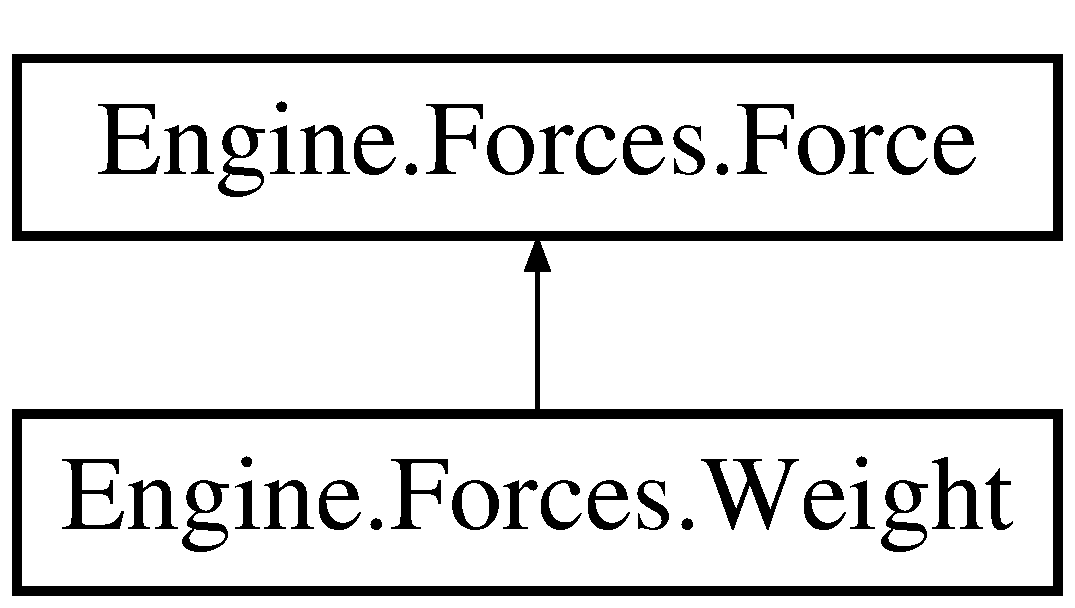
\includegraphics[height=2.000000cm]{class_engine_1_1_forces_1_1_weight}
\end{center}
\end{figure}
\subsection*{Public Member Functions}
\begin{DoxyCompactItemize}
\item 
{\bf Weight} ()
\item 
{\bf Weight} (double weight)
\end{DoxyCompactItemize}


\subsection{Detailed Description}
Created by IntelliJ IDEA. User: Sina Solaimanpour Date: 10/18/11 Time: 10:47 PM 

\subsection{Constructor \& Destructor Documentation}
\index{Engine::Forces::Weight@{Engine::Forces::Weight}!Weight@{Weight}}
\index{Weight@{Weight}!Engine::Forces::Weight@{Engine::Forces::Weight}}
\subsubsection[{Weight}]{\setlength{\rightskip}{0pt plus 5cm}Engine.Forces.Weight.Weight (
\begin{DoxyParamCaption}
{}
\end{DoxyParamCaption}
)}\label{class_engine_1_1_forces_1_1_weight_a77373a754644f9adc47adc9fa8ccf38d}
Default Constructor, It Sets The X \doxyref{Force}{p.}{class_engine_1_1_forces_1_1_force} 0 so that weight get simulated properly and It will set The Y \doxyref{Force}{p.}{class_engine_1_1_forces_1_1_force} 10 just for fun \index{Engine::Forces::Weight@{Engine::Forces::Weight}!Weight@{Weight}}
\index{Weight@{Weight}!Engine::Forces::Weight@{Engine::Forces::Weight}}
\subsubsection[{Weight}]{\setlength{\rightskip}{0pt plus 5cm}Engine.Forces.Weight.Weight (
\begin{DoxyParamCaption}
\item[{double}]{ weight}
\end{DoxyParamCaption}
)}\label{class_engine_1_1_forces_1_1_weight_a62b8ccef36782477db6a39a3e86bc4fe}
It Sets The X \doxyref{Force}{p.}{class_engine_1_1_forces_1_1_force} 0 so that weight get simulated properly and It will set The Y \doxyref{Force}{p.}{class_engine_1_1_forces_1_1_force} to parameter passed by user


\begin{DoxyParams}{Parameters}
\item[{\em weight}]For The Y \doxyref{Force}{p.}{class_engine_1_1_forces_1_1_force} Value \end{DoxyParams}


The documentation for this class was generated from the following file:\begin{DoxyCompactItemize}
\item 
src/Engine/Forces/Weight.java\end{DoxyCompactItemize}

\section{Engine.Forces.Wind Class Reference}
\label{class_engine_1_1_forces_1_1_wind}\index{Engine::Forces::Wind@{Engine::Forces::Wind}}
Inheritance diagram for Engine.Forces.Wind:\begin{figure}[H]
\begin{center}
\leavevmode
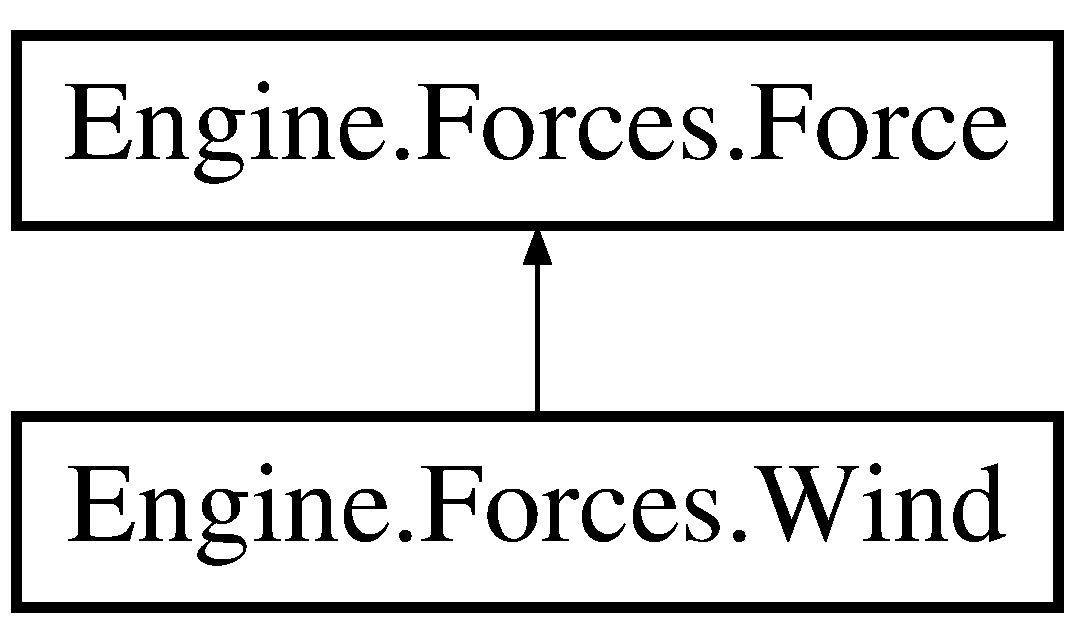
\includegraphics[height=2.000000cm]{class_engine_1_1_forces_1_1_wind}
\end{center}
\end{figure}
\subsection*{Public Member Functions}
\begin{DoxyCompactItemize}
\item 
{\bf Wind} (double power, double angle)
\end{DoxyCompactItemize}


\subsection{Detailed Description}
Created by IntelliJ IDEA. User: Sina Date: 10/22/11 Time: 11:40 AM To change this template use File $|$ Settings $|$ File Templates. 

\subsection{Constructor \& Destructor Documentation}
\index{Engine::Forces::Wind@{Engine::Forces::Wind}!Wind@{Wind}}
\index{Wind@{Wind}!Engine::Forces::Wind@{Engine::Forces::Wind}}
\subsubsection[{Wind}]{\setlength{\rightskip}{0pt plus 5cm}Engine.Forces.Wind.Wind (
\begin{DoxyParamCaption}
\item[{double}]{ power, }
\item[{double}]{ angle}
\end{DoxyParamCaption}
)}\label{class_engine_1_1_forces_1_1_wind_a809b9e35bdd73dbfa5cacde290ef0192}
This Will Create a \doxyref{Force}{p.}{class_engine_1_1_forces_1_1_force} Object as \doxyref{Wind}{p.}{class_engine_1_1_forces_1_1_wind} with the power and angle passed to the constructor


\begin{DoxyParams}{Parameters}
\item[{\em power}]Power of the \doxyref{Wind}{p.}{class_engine_1_1_forces_1_1_wind} \item[{\em angle}]Angle og the \doxyref{Wind}{p.}{class_engine_1_1_forces_1_1_wind} \end{DoxyParams}


The documentation for this class was generated from the following file:\begin{DoxyCompactItemize}
\item 
src/Engine/Forces/Wind.java\end{DoxyCompactItemize}

\section{Engine.World.World Class Reference}
\label{class_engine_1_1_world_1_1_world}\index{Engine::World::World@{Engine::World::World}}
\subsection*{Public Member Functions}
\begin{DoxyCompactItemize}
\item 
void {\bf addCollisionListener} ({\bf CollisionListener} listener)
\item 
void {\bf removeCollisionListener} ({\bf CollisionListener} listener)
\item 
{\bf World} ()
\item 
{\bf World} (double gravity, boolean ceil, boolean ground, boolean leftWall, boolean rightWall, int width, int height, int scale, JFrame frame)
\item 
{\bf World} (double gravity, int scale, int width, int height, JFrame frame)
\item 
void {\bf updateObject} ({\bf Object2D} obj)
\item 
void {\bf drawScale} (Graphics2D g)
\item 
void {\bf updateWorld} ()
\item 
Double[$\,$] {\bf projectObject} ({\bf Vector2D} axis, {\bf RectangularObject} obj)
\item 
Double[$\,$] {\bf projectObject} ({\bf Vector2D} axis, {\bf CircularObject} obj)
\item 
double {\bf IntervalDistance} (double minA, double maxA, double minB, double maxB)
\item 
void {\bf setDefaultFrame} (JFrame defaultFrame)
\item 
void {\bf addObject} ({\bf Object2D} obj)
\item 
double {\bf getWindPower} ()
\item 
void {\bf setWindPower} (double windPower)
\item 
double {\bf getWindAngle} ()
\item 
void {\bf setWindAngle} (double windAngle)
\item 
double {\bf getTimeStep} ()
\item 
void {\bf setTimeStep} (int timeStep)
\item 
JFrame {\bf getDefaultFrame} ()
\item 
double {\bf getGravity} ()
\item 
void {\bf setGravity} (double gravity)
\item 
Timer {\bf getClock} ()
\item 
void {\bf setClock} (Timer clock)
\item 
boolean {\bf isCeil} ()
\item 
void {\bf setCeil} (boolean ceil)
\item 
boolean {\bf isGround} ()
\item 
void {\bf setGround} (boolean ground)
\item 
boolean {\bf isLeftWall} ()
\item 
void {\bf setLeftWall} (boolean leftWall)
\item 
boolean {\bf isRightWall} ()
\item 
void {\bf setRightWall} (boolean rightWall)
\item 
List$<$ {\bf Object2D} $>$ {\bf getObjects} ()
\item 
int {\bf getScale} ()
\item 
void {\bf setScale} (int scale)
\item 
int {\bf getWidth} ()
\item 
void {\bf setWidth} (int width)
\item 
int {\bf getHeight} ()
\item 
void {\bf setHeight} (int height)
\item 
Canvas {\bf getWorldCanvas} ()
\item 
void {\bf setWorldCanvas} (Canvas worldCanvas)
\item 
boolean {\bf isLeaveShadow} ()
\item 
void {\bf setLeaveShadow} (boolean leaveShadow)
\end{DoxyCompactItemize}
\subsection*{Protected Attributes}
\begin{DoxyCompactItemize}
\item 
javax.swing.event.EventListenerList {\bf listenerList} = new javax.swing.event.EventListenerList()
\end{DoxyCompactItemize}
\subsection*{Package Functions}
\begin{DoxyCompactItemize}
\item 
void {\bf fireCollisionEvent} ({\bf CollisionEvent} evt)
\end{DoxyCompactItemize}
\subsection*{Package Attributes}
\begin{DoxyCompactItemize}
\item 
double {\bfseries gravity} = 0.98\label{class_engine_1_1_world_1_1_world_a325dacf5546bf2573cca5c37f052015d}

\item 
double {\bfseries windPower} = 0\label{class_engine_1_1_world_1_1_world_a32d1bba862c7aa187da584705e19cd85}

\item 
double {\bfseries windAngle} = 0\label{class_engine_1_1_world_1_1_world_a435db6f8ab2eac447c228295edab306e}

\item 
Timer {\bfseries clock} = new Timer()\label{class_engine_1_1_world_1_1_world_a6061e1e0566b91e8870dd62d84301aa4}

\item 
boolean {\bfseries ceil} = true\label{class_engine_1_1_world_1_1_world_aadc1c4305f9235f44abc8286139dd2b2}

\item 
boolean {\bfseries ground} = true\label{class_engine_1_1_world_1_1_world_acfab8905c98c83af71b26cfec265642f}

\item 
boolean {\bfseries leftWall} = true\label{class_engine_1_1_world_1_1_world_ad9388f768ba4891ce20232231b0113a8}

\item 
boolean {\bfseries rightWall} = true\label{class_engine_1_1_world_1_1_world_a103937e2f8ba6d14136b96348a01d4d4}

\item 
List$<$ {\bf Object2D} $>$ {\bfseries objects} = new ArrayList$<${\bf Object2D}$>$()\label{class_engine_1_1_world_1_1_world_a2903968632a0072a5107ee051b35eb81}

\item 
List$<$ {\bf Object2D} $>$ {\bfseries rotatingObjects} = new ArrayList$<${\bf Object2D}$>$()\label{class_engine_1_1_world_1_1_world_ac3874d7a710ac634612bf09ed8084308}

\item 
int {\bfseries scale} = 50\label{class_engine_1_1_world_1_1_world_a76a4e8d16c3c01adb49b517c33221df9}

\item 
int {\bfseries width}\label{class_engine_1_1_world_1_1_world_a3ee2f77aca754151705e6719710720d4}

\item 
int {\bfseries height}\label{class_engine_1_1_world_1_1_world_aa9ef92230266992d3e328ee67674c0a8}

\item 
double {\bfseries timeStep} = {\bf Properties.timeStep}\label{class_engine_1_1_world_1_1_world_ad3249b2e3f5e6d328591c72214e5924a}

\item 
JFrame {\bfseries defaultFrame}\label{class_engine_1_1_world_1_1_world_a9bcfb6a34b93ea6d4dbb54bbff10e713}

\item 
Canvas {\bfseries worldCanvas}\label{class_engine_1_1_world_1_1_world_ac95714d63363d98d664ce2e89680c0be}

\item 
BufferStrategy {\bfseries strategy}\label{class_engine_1_1_world_1_1_world_a70a113725642db22c38cb3f013e3be03}

\item 
boolean {\bfseries leaveShadow} = false\label{class_engine_1_1_world_1_1_world_abd29ac6c49124e64ed0846d9271b7519}

\end{DoxyCompactItemize}


\subsection{Detailed Description}
Created by IntelliJ IDEA. User: Sina Solaimanpour Date: 10/18/11 Time: 10:43 PM 

\subsection{Constructor \& Destructor Documentation}
\index{Engine::World::World@{Engine::World::World}!World@{World}}
\index{World@{World}!Engine::World::World@{Engine::World::World}}
\subsubsection[{World}]{\setlength{\rightskip}{0pt plus 5cm}Engine.World.World.World (
\begin{DoxyParamCaption}
{}
\end{DoxyParamCaption}
)}\label{class_engine_1_1_world_1_1_world_ae985ae6c588006c1a7e89e4c204e4af8}
constructor of world \index{Engine::World::World@{Engine::World::World}!World@{World}}
\index{World@{World}!Engine::World::World@{Engine::World::World}}
\subsubsection[{World}]{\setlength{\rightskip}{0pt plus 5cm}Engine.World.World.World (
\begin{DoxyParamCaption}
\item[{double}]{ gravity, }
\item[{boolean}]{ ceil, }
\item[{boolean}]{ ground, }
\item[{boolean}]{ leftWall, }
\item[{boolean}]{ rightWall, }
\item[{int}]{ width, }
\item[{int}]{ height, }
\item[{int}]{ scale, }
\item[{JFrame}]{ frame}
\end{DoxyParamCaption}
)}\label{class_engine_1_1_world_1_1_world_a5c107188952b8cec978064346d201c9e}
main constructor of world


\begin{DoxyParams}{Parameters}
\item[{\em gravity}]gravity of the world \item[{\em ceil}]it indicates that our world has ceil or not \item[{\em ground}]it indicates that our world has ground or not \item[{\em leftWall}]it indicates that our world has leftWall or not \item[{\em rightWall}]it indicates that our world has rightWall or not \item[{\em width}]width of world \item[{\em height}]height of world \item[{\em scale}]scale of world \item[{\em frame}]frame of world \end{DoxyParams}
\index{Engine::World::World@{Engine::World::World}!World@{World}}
\index{World@{World}!Engine::World::World@{Engine::World::World}}
\subsubsection[{World}]{\setlength{\rightskip}{0pt plus 5cm}Engine.World.World.World (
\begin{DoxyParamCaption}
\item[{double}]{ gravity, }
\item[{int}]{ scale, }
\item[{int}]{ width, }
\item[{int}]{ height, }
\item[{JFrame}]{ frame}
\end{DoxyParamCaption}
)}\label{class_engine_1_1_world_1_1_world_aca11a205b9dd182ff8d5459f1323f867}
constructor of world


\begin{DoxyParams}{Parameters}
\item[{\em gravity}]gravity of the world \item[{\em scale}]scale of world \item[{\em width}]width of world \item[{\em height}]height of world \item[{\em frame}]frame of world \end{DoxyParams}


\subsection{Member Function Documentation}
\index{Engine::World::World@{Engine::World::World}!addCollisionListener@{addCollisionListener}}
\index{addCollisionListener@{addCollisionListener}!Engine::World::World@{Engine::World::World}}
\subsubsection[{addCollisionListener}]{\setlength{\rightskip}{0pt plus 5cm}void Engine.World.World.addCollisionListener (
\begin{DoxyParamCaption}
\item[{{\bf CollisionListener}}]{ listener}
\end{DoxyParamCaption}
)}\label{class_engine_1_1_world_1_1_world_acf24ea729ba52441e1ec79e0b8f8b81e}
adds a collision listener to world


\begin{DoxyParams}{Parameters}
\item[{\em listener}]the listener that is going to be added to the world \end{DoxyParams}
\index{Engine::World::World@{Engine::World::World}!addObject@{addObject}}
\index{addObject@{addObject}!Engine::World::World@{Engine::World::World}}
\subsubsection[{addObject}]{\setlength{\rightskip}{0pt plus 5cm}void Engine.World.World.addObject (
\begin{DoxyParamCaption}
\item[{{\bf Object2D}}]{ obj}
\end{DoxyParamCaption}
)}\label{class_engine_1_1_world_1_1_world_a93c3d4e79f770021ba12317d9632fe7d}
adds a object to the world


\begin{DoxyParams}{Parameters}
\item[{\em obj}]the object that will be added to world \end{DoxyParams}
\index{Engine::World::World@{Engine::World::World}!drawScale@{drawScale}}
\index{drawScale@{drawScale}!Engine::World::World@{Engine::World::World}}
\subsubsection[{drawScale}]{\setlength{\rightskip}{0pt plus 5cm}void Engine.World.World.drawScale (
\begin{DoxyParamCaption}
\item[{Graphics2D}]{ g}
\end{DoxyParamCaption}
)}\label{class_engine_1_1_world_1_1_world_a3cd7ae940554c4e8f59a56494681cb29}
draws the scale on the screen


\begin{DoxyParams}{Parameters}
\item[{\em g}]graphics2D object of screen \end{DoxyParams}
\index{Engine::World::World@{Engine::World::World}!fireCollisionEvent@{fireCollisionEvent}}
\index{fireCollisionEvent@{fireCollisionEvent}!Engine::World::World@{Engine::World::World}}
\subsubsection[{fireCollisionEvent}]{\setlength{\rightskip}{0pt plus 5cm}void Engine.World.World.fireCollisionEvent (
\begin{DoxyParamCaption}
\item[{{\bf CollisionEvent}}]{ evt}
\end{DoxyParamCaption}
)\hspace{0.3cm}{\ttfamily  [package]}}\label{class_engine_1_1_world_1_1_world_adbd7c85d03270ec42ea9f9a48eec563a}
indicates that the event is happened


\begin{DoxyParams}{Parameters}
\item[{\em evt}]event that is happened \end{DoxyParams}
\index{Engine::World::World@{Engine::World::World}!getClock@{getClock}}
\index{getClock@{getClock}!Engine::World::World@{Engine::World::World}}
\subsubsection[{getClock}]{\setlength{\rightskip}{0pt plus 5cm}Timer Engine.World.World.getClock (
\begin{DoxyParamCaption}
{}
\end{DoxyParamCaption}
)}\label{class_engine_1_1_world_1_1_world_ae75a94d60a2aee8992702b9eaffd9e12}
return the clock of world

\begin{DoxyReturn}{Returns}
clock of world 
\end{DoxyReturn}
\index{Engine::World::World@{Engine::World::World}!getDefaultFrame@{getDefaultFrame}}
\index{getDefaultFrame@{getDefaultFrame}!Engine::World::World@{Engine::World::World}}
\subsubsection[{getDefaultFrame}]{\setlength{\rightskip}{0pt plus 5cm}JFrame Engine.World.World.getDefaultFrame (
\begin{DoxyParamCaption}
{}
\end{DoxyParamCaption}
)}\label{class_engine_1_1_world_1_1_world_a3175705ca1c7bc7bdbdfafd387df3591}
returns the default frame of world

\begin{DoxyReturn}{Returns}
default frame of world 
\end{DoxyReturn}
\index{Engine::World::World@{Engine::World::World}!getGravity@{getGravity}}
\index{getGravity@{getGravity}!Engine::World::World@{Engine::World::World}}
\subsubsection[{getGravity}]{\setlength{\rightskip}{0pt plus 5cm}double Engine.World.World.getGravity (
\begin{DoxyParamCaption}
{}
\end{DoxyParamCaption}
)}\label{class_engine_1_1_world_1_1_world_a8c58808e3d6a34ee1a83843cb66657d8}
returns the gravity of world

\begin{DoxyReturn}{Returns}
gravity of world 
\end{DoxyReturn}
\index{Engine::World::World@{Engine::World::World}!getHeight@{getHeight}}
\index{getHeight@{getHeight}!Engine::World::World@{Engine::World::World}}
\subsubsection[{getHeight}]{\setlength{\rightskip}{0pt plus 5cm}int Engine.World.World.getHeight (
\begin{DoxyParamCaption}
{}
\end{DoxyParamCaption}
)}\label{class_engine_1_1_world_1_1_world_a8e9c9e5f93d78637b3af218c2bc36a39}
access the height of world

\begin{DoxyReturn}{Returns}
height of the world 
\end{DoxyReturn}
\index{Engine::World::World@{Engine::World::World}!getObjects@{getObjects}}
\index{getObjects@{getObjects}!Engine::World::World@{Engine::World::World}}
\subsubsection[{getObjects}]{\setlength{\rightskip}{0pt plus 5cm}List$<${\bf Object2D}$>$ Engine.World.World.getObjects (
\begin{DoxyParamCaption}
{}
\end{DoxyParamCaption}
)}\label{class_engine_1_1_world_1_1_world_a57790bc2b24b92a4625e6f49ef25f2c0}
to access all of the worlds objects

\begin{DoxyReturn}{Returns}
returns the list of all worlds objects 
\end{DoxyReturn}
\index{Engine::World::World@{Engine::World::World}!getScale@{getScale}}
\index{getScale@{getScale}!Engine::World::World@{Engine::World::World}}
\subsubsection[{getScale}]{\setlength{\rightskip}{0pt plus 5cm}int Engine.World.World.getScale (
\begin{DoxyParamCaption}
{}
\end{DoxyParamCaption}
)}\label{class_engine_1_1_world_1_1_world_ae6ca31807c3ddea0e80bfb48740fdaa4}
to access the scale value of the world (the pixel numbers of one meter)

\begin{DoxyReturn}{Returns}
the scale value for this world 
\end{DoxyReturn}
\index{Engine::World::World@{Engine::World::World}!getTimeStep@{getTimeStep}}
\index{getTimeStep@{getTimeStep}!Engine::World::World@{Engine::World::World}}
\subsubsection[{getTimeStep}]{\setlength{\rightskip}{0pt plus 5cm}double Engine.World.World.getTimeStep (
\begin{DoxyParamCaption}
{}
\end{DoxyParamCaption}
)}\label{class_engine_1_1_world_1_1_world_a92fa828361e8e6f73efdd43b995615c9}
returns the timestep of world

\begin{DoxyReturn}{Returns}
timestep of world 
\end{DoxyReturn}
\index{Engine::World::World@{Engine::World::World}!getWidth@{getWidth}}
\index{getWidth@{getWidth}!Engine::World::World@{Engine::World::World}}
\subsubsection[{getWidth}]{\setlength{\rightskip}{0pt plus 5cm}int Engine.World.World.getWidth (
\begin{DoxyParamCaption}
{}
\end{DoxyParamCaption}
)}\label{class_engine_1_1_world_1_1_world_aecbbb6746ac8169b1bdd6c1e80462064}
access the width of world

\begin{DoxyReturn}{Returns}
width of the world 
\end{DoxyReturn}
\index{Engine::World::World@{Engine::World::World}!getWindAngle@{getWindAngle}}
\index{getWindAngle@{getWindAngle}!Engine::World::World@{Engine::World::World}}
\subsubsection[{getWindAngle}]{\setlength{\rightskip}{0pt plus 5cm}double Engine.World.World.getWindAngle (
\begin{DoxyParamCaption}
{}
\end{DoxyParamCaption}
)}\label{class_engine_1_1_world_1_1_world_ac9154c8e14ee146465f38988ca1b08ed}
returns the wind angle of world

\begin{DoxyReturn}{Returns}
wind angle of world 
\end{DoxyReturn}
\index{Engine::World::World@{Engine::World::World}!getWindPower@{getWindPower}}
\index{getWindPower@{getWindPower}!Engine::World::World@{Engine::World::World}}
\subsubsection[{getWindPower}]{\setlength{\rightskip}{0pt plus 5cm}double Engine.World.World.getWindPower (
\begin{DoxyParamCaption}
{}
\end{DoxyParamCaption}
)}\label{class_engine_1_1_world_1_1_world_acd85055d453c9977077544d98f335e3e}
returns the wind power of world

\begin{DoxyReturn}{Returns}
wind power of world 
\end{DoxyReturn}
\index{Engine::World::World@{Engine::World::World}!getWorldCanvas@{getWorldCanvas}}
\index{getWorldCanvas@{getWorldCanvas}!Engine::World::World@{Engine::World::World}}
\subsubsection[{getWorldCanvas}]{\setlength{\rightskip}{0pt plus 5cm}Canvas Engine.World.World.getWorldCanvas (
\begin{DoxyParamCaption}
{}
\end{DoxyParamCaption}
)}\label{class_engine_1_1_world_1_1_world_a402c25bf60ecfeb1820a5c3e203f49c1}
worlds canvas

\begin{DoxyReturn}{Returns}
worlds canvas 
\end{DoxyReturn}
\index{Engine::World::World@{Engine::World::World}!IntervalDistance@{IntervalDistance}}
\index{IntervalDistance@{IntervalDistance}!Engine::World::World@{Engine::World::World}}
\subsubsection[{IntervalDistance}]{\setlength{\rightskip}{0pt plus 5cm}double Engine.World.World.IntervalDistance (
\begin{DoxyParamCaption}
\item[{double}]{ minA, }
\item[{double}]{ maxA, }
\item[{double}]{ minB, }
\item[{double}]{ maxB}
\end{DoxyParamCaption}
)}\label{class_engine_1_1_world_1_1_world_a60f6b6772fd1c083c8cc40e306d44bb3}
Calculate the distance between [minA, maxA] and [minB, maxB] ,The distance will be negative if the intervals overlap


\begin{DoxyParams}{Parameters}
\item[{\em minA}]minimum position of objectA's projection area \item[{\em maxA}]maximum position of objectA's projection area \item[{\em minB}]minimum position of objectB's projection area \item[{\em maxB}]maximum position of objectB's projection area \end{DoxyParams}
\begin{DoxyReturn}{Returns}
interval between two projection areas 
\end{DoxyReturn}
\index{Engine::World::World@{Engine::World::World}!isCeil@{isCeil}}
\index{isCeil@{isCeil}!Engine::World::World@{Engine::World::World}}
\subsubsection[{isCeil}]{\setlength{\rightskip}{0pt plus 5cm}boolean Engine.World.World.isCeil (
\begin{DoxyParamCaption}
{}
\end{DoxyParamCaption}
)}\label{class_engine_1_1_world_1_1_world_a45e2371f412e6a653f1888f1e5678b00}
return true if the world has ceil

\begin{DoxyReturn}{Returns}
boolean ceil 
\end{DoxyReturn}
\index{Engine::World::World@{Engine::World::World}!isGround@{isGround}}
\index{isGround@{isGround}!Engine::World::World@{Engine::World::World}}
\subsubsection[{isGround}]{\setlength{\rightskip}{0pt plus 5cm}boolean Engine.World.World.isGround (
\begin{DoxyParamCaption}
{}
\end{DoxyParamCaption}
)}\label{class_engine_1_1_world_1_1_world_a79e402f7dbf2ae2e03623f18c9fa5763}
return true if the world has ground

\begin{DoxyReturn}{Returns}
boolean ground 
\end{DoxyReturn}
\index{Engine::World::World@{Engine::World::World}!isLeaveShadow@{isLeaveShadow}}
\index{isLeaveShadow@{isLeaveShadow}!Engine::World::World@{Engine::World::World}}
\subsubsection[{isLeaveShadow}]{\setlength{\rightskip}{0pt plus 5cm}boolean Engine.World.World.isLeaveShadow (
\begin{DoxyParamCaption}
{}
\end{DoxyParamCaption}
)}\label{class_engine_1_1_world_1_1_world_a5df0cb6b77c4b2a659bf844b6ca7239f}
\begin{DoxyReturn}{Returns}
Checks if The \doxyref{World}{p.}{class_engine_1_1_world_1_1_world} Leaves Shadow or Not 
\end{DoxyReturn}
\index{Engine::World::World@{Engine::World::World}!isLeftWall@{isLeftWall}}
\index{isLeftWall@{isLeftWall}!Engine::World::World@{Engine::World::World}}
\subsubsection[{isLeftWall}]{\setlength{\rightskip}{0pt plus 5cm}boolean Engine.World.World.isLeftWall (
\begin{DoxyParamCaption}
{}
\end{DoxyParamCaption}
)}\label{class_engine_1_1_world_1_1_world_a0ada7079911c4529f2e90e9807a0a499}
returns true if the world has left wall

\begin{DoxyReturn}{Returns}
boolean left wall 
\end{DoxyReturn}
\index{Engine::World::World@{Engine::World::World}!isRightWall@{isRightWall}}
\index{isRightWall@{isRightWall}!Engine::World::World@{Engine::World::World}}
\subsubsection[{isRightWall}]{\setlength{\rightskip}{0pt plus 5cm}boolean Engine.World.World.isRightWall (
\begin{DoxyParamCaption}
{}
\end{DoxyParamCaption}
)}\label{class_engine_1_1_world_1_1_world_aa1539e44a7aaa72e06f77e7d9039cd65}
returns true if the world has right wall

\begin{DoxyReturn}{Returns}
boolean right wall 
\end{DoxyReturn}
\index{Engine::World::World@{Engine::World::World}!projectObject@{projectObject}}
\index{projectObject@{projectObject}!Engine::World::World@{Engine::World::World}}
\subsubsection[{projectObject}]{\setlength{\rightskip}{0pt plus 5cm}Double [$\,$] Engine.World.World.projectObject (
\begin{DoxyParamCaption}
\item[{{\bf Vector2D}}]{ axis, }
\item[{{\bf CircularObject}}]{ obj}
\end{DoxyParamCaption}
)}\label{class_engine_1_1_world_1_1_world_ade19534358d8162163d0ce09d8c97270}
Calculates the projection of a circular object on an axis and returns it as a [min, max] interval


\begin{DoxyParams}{Parameters}
\item[{\em axis}]the axis that projction applies to \item[{\em obj}]object that will be projected to the axis \end{DoxyParams}
\begin{DoxyReturn}{Returns}
min and max of projected area 
\end{DoxyReturn}
\index{Engine::World::World@{Engine::World::World}!projectObject@{projectObject}}
\index{projectObject@{projectObject}!Engine::World::World@{Engine::World::World}}
\subsubsection[{projectObject}]{\setlength{\rightskip}{0pt plus 5cm}Double [$\,$] Engine.World.World.projectObject (
\begin{DoxyParamCaption}
\item[{{\bf Vector2D}}]{ axis, }
\item[{{\bf RectangularObject}}]{ obj}
\end{DoxyParamCaption}
)}\label{class_engine_1_1_world_1_1_world_ac17d61500d5576bd21ba547ed3e5e64c}
Calculates the projection of a rectangular object on an axis and returns it as a [min, max] interval


\begin{DoxyParams}{Parameters}
\item[{\em axis}]the axis that projction applies to \item[{\em obj}]object that will be projected to the axis \end{DoxyParams}
\begin{DoxyReturn}{Returns}
min and max of projected area 
\end{DoxyReturn}
\index{Engine::World::World@{Engine::World::World}!removeCollisionListener@{removeCollisionListener}}
\index{removeCollisionListener@{removeCollisionListener}!Engine::World::World@{Engine::World::World}}
\subsubsection[{removeCollisionListener}]{\setlength{\rightskip}{0pt plus 5cm}void Engine.World.World.removeCollisionListener (
\begin{DoxyParamCaption}
\item[{{\bf CollisionListener}}]{ listener}
\end{DoxyParamCaption}
)}\label{class_engine_1_1_world_1_1_world_a2d91b37b9e55b76eecf1928466c42674}
removes a collision listener from world


\begin{DoxyParams}{Parameters}
\item[{\em listener}]the listener that is going to be removed from the world \end{DoxyParams}
\index{Engine::World::World@{Engine::World::World}!setCeil@{setCeil}}
\index{setCeil@{setCeil}!Engine::World::World@{Engine::World::World}}
\subsubsection[{setCeil}]{\setlength{\rightskip}{0pt plus 5cm}void Engine.World.World.setCeil (
\begin{DoxyParamCaption}
\item[{boolean}]{ ceil}
\end{DoxyParamCaption}
)}\label{class_engine_1_1_world_1_1_world_aad7d81b3fa732a2d1329450f6bfb13ec}
sets the ceil boolean to assign ceil to world


\begin{DoxyParams}{Parameters}
\item[{\em ceil}]boolean value for ceil if true the world has ceil \end{DoxyParams}
\index{Engine::World::World@{Engine::World::World}!setClock@{setClock}}
\index{setClock@{setClock}!Engine::World::World@{Engine::World::World}}
\subsubsection[{setClock}]{\setlength{\rightskip}{0pt plus 5cm}void Engine.World.World.setClock (
\begin{DoxyParamCaption}
\item[{Timer}]{ clock}
\end{DoxyParamCaption}
)}\label{class_engine_1_1_world_1_1_world_a29a3fffe8b2016c15c9d3242f2387cc8}
sets the clock of world


\begin{DoxyParams}{Parameters}
\item[{\em clock}]clock to set to world \end{DoxyParams}
\index{Engine::World::World@{Engine::World::World}!setDefaultFrame@{setDefaultFrame}}
\index{setDefaultFrame@{setDefaultFrame}!Engine::World::World@{Engine::World::World}}
\subsubsection[{setDefaultFrame}]{\setlength{\rightskip}{0pt plus 5cm}void Engine.World.World.setDefaultFrame (
\begin{DoxyParamCaption}
\item[{JFrame}]{ defaultFrame}
\end{DoxyParamCaption}
)}\label{class_engine_1_1_world_1_1_world_a7c05e213d884e46e5f034fe55f128c85}
sets the frame of the world


\begin{DoxyParams}{Parameters}
\item[{\em defaultFrame}]the frame that is going to be set to the world \end{DoxyParams}
\index{Engine::World::World@{Engine::World::World}!setGravity@{setGravity}}
\index{setGravity@{setGravity}!Engine::World::World@{Engine::World::World}}
\subsubsection[{setGravity}]{\setlength{\rightskip}{0pt plus 5cm}void Engine.World.World.setGravity (
\begin{DoxyParamCaption}
\item[{double}]{ gravity}
\end{DoxyParamCaption}
)}\label{class_engine_1_1_world_1_1_world_af9c4d12d62176b880ed37d4a9df70d22}
sets the gravity


\begin{DoxyParams}{Parameters}
\item[{\em gravity}]gravity to set to world \end{DoxyParams}
\index{Engine::World::World@{Engine::World::World}!setGround@{setGround}}
\index{setGround@{setGround}!Engine::World::World@{Engine::World::World}}
\subsubsection[{setGround}]{\setlength{\rightskip}{0pt plus 5cm}void Engine.World.World.setGround (
\begin{DoxyParamCaption}
\item[{boolean}]{ ground}
\end{DoxyParamCaption}
)}\label{class_engine_1_1_world_1_1_world_a9bdeb81b505fab3c9a3edbb1b4a78cd6}
sets the ground boolean to assign ground to world


\begin{DoxyParams}{Parameters}
\item[{\em ground}]boolean value for ground if true the world has ground \end{DoxyParams}
\index{Engine::World::World@{Engine::World::World}!setHeight@{setHeight}}
\index{setHeight@{setHeight}!Engine::World::World@{Engine::World::World}}
\subsubsection[{setHeight}]{\setlength{\rightskip}{0pt plus 5cm}void Engine.World.World.setHeight (
\begin{DoxyParamCaption}
\item[{int}]{ height}
\end{DoxyParamCaption}
)}\label{class_engine_1_1_world_1_1_world_af1f7684016e5c03222ebb6d805657591}
sets the heights of world


\begin{DoxyParams}{Parameters}
\item[{\em height}]of the world \end{DoxyParams}
\index{Engine::World::World@{Engine::World::World}!setLeaveShadow@{setLeaveShadow}}
\index{setLeaveShadow@{setLeaveShadow}!Engine::World::World@{Engine::World::World}}
\subsubsection[{setLeaveShadow}]{\setlength{\rightskip}{0pt plus 5cm}void Engine.World.World.setLeaveShadow (
\begin{DoxyParamCaption}
\item[{boolean}]{ leaveShadow}
\end{DoxyParamCaption}
)}\label{class_engine_1_1_world_1_1_world_a3ab3e6dcd519a78ca03bd4684829378f}

\begin{DoxyParams}{Parameters}
\item[{\em leaveShadow}]Sets The leaveShadow Property (if true the world would not be cleared on each update) \end{DoxyParams}
\index{Engine::World::World@{Engine::World::World}!setLeftWall@{setLeftWall}}
\index{setLeftWall@{setLeftWall}!Engine::World::World@{Engine::World::World}}
\subsubsection[{setLeftWall}]{\setlength{\rightskip}{0pt plus 5cm}void Engine.World.World.setLeftWall (
\begin{DoxyParamCaption}
\item[{boolean}]{ leftWall}
\end{DoxyParamCaption}
)}\label{class_engine_1_1_world_1_1_world_a3f23c7180a71101cc0ffa642f167e5e1}
sets the left wall boolean to assign left wall to world


\begin{DoxyParams}{Parameters}
\item[{\em leftWall}]boolean value for left wall if true the world has left wall \end{DoxyParams}
\index{Engine::World::World@{Engine::World::World}!setRightWall@{setRightWall}}
\index{setRightWall@{setRightWall}!Engine::World::World@{Engine::World::World}}
\subsubsection[{setRightWall}]{\setlength{\rightskip}{0pt plus 5cm}void Engine.World.World.setRightWall (
\begin{DoxyParamCaption}
\item[{boolean}]{ rightWall}
\end{DoxyParamCaption}
)}\label{class_engine_1_1_world_1_1_world_aaa1f3efb47fa5dc308682c10d4a8beb5}
sets the right wall boolean to assign left wall to world


\begin{DoxyParams}{Parameters}
\item[{\em rightWall}]boolean value for right wall if true the world has right wall \end{DoxyParams}
\index{Engine::World::World@{Engine::World::World}!setScale@{setScale}}
\index{setScale@{setScale}!Engine::World::World@{Engine::World::World}}
\subsubsection[{setScale}]{\setlength{\rightskip}{0pt plus 5cm}void Engine.World.World.setScale (
\begin{DoxyParamCaption}
\item[{int}]{ scale}
\end{DoxyParamCaption}
)}\label{class_engine_1_1_world_1_1_world_a7546c8fc35f880d5ce84f2bb6da0637b}
sets the scale value for the world


\begin{DoxyParams}{Parameters}
\item[{\em scale}]scale value for this world \end{DoxyParams}
\index{Engine::World::World@{Engine::World::World}!setTimeStep@{setTimeStep}}
\index{setTimeStep@{setTimeStep}!Engine::World::World@{Engine::World::World}}
\subsubsection[{setTimeStep}]{\setlength{\rightskip}{0pt plus 5cm}void Engine.World.World.setTimeStep (
\begin{DoxyParamCaption}
\item[{int}]{ timeStep}
\end{DoxyParamCaption}
)}\label{class_engine_1_1_world_1_1_world_af312fb3dfd22a5f5a4951e0ce84491ab}
sets the timestep


\begin{DoxyParams}{Parameters}
\item[{\em timeStep}]timestep to set to world \end{DoxyParams}
\index{Engine::World::World@{Engine::World::World}!setWidth@{setWidth}}
\index{setWidth@{setWidth}!Engine::World::World@{Engine::World::World}}
\subsubsection[{setWidth}]{\setlength{\rightskip}{0pt plus 5cm}void Engine.World.World.setWidth (
\begin{DoxyParamCaption}
\item[{int}]{ width}
\end{DoxyParamCaption}
)}\label{class_engine_1_1_world_1_1_world_a1b42e3ad5604e50af52a4fbc8bebf5fe}
sets the width of world


\begin{DoxyParams}{Parameters}
\item[{\em width}]of the world \end{DoxyParams}
\index{Engine::World::World@{Engine::World::World}!setWindAngle@{setWindAngle}}
\index{setWindAngle@{setWindAngle}!Engine::World::World@{Engine::World::World}}
\subsubsection[{setWindAngle}]{\setlength{\rightskip}{0pt plus 5cm}void Engine.World.World.setWindAngle (
\begin{DoxyParamCaption}
\item[{double}]{ windAngle}
\end{DoxyParamCaption}
)}\label{class_engine_1_1_world_1_1_world_a0421e8ba8d485565415ca86890c4d7de}
sets the wind angle


\begin{DoxyParams}{Parameters}
\item[{\em windAngle}]wind angle to set to world \end{DoxyParams}
\index{Engine::World::World@{Engine::World::World}!setWindPower@{setWindPower}}
\index{setWindPower@{setWindPower}!Engine::World::World@{Engine::World::World}}
\subsubsection[{setWindPower}]{\setlength{\rightskip}{0pt plus 5cm}void Engine.World.World.setWindPower (
\begin{DoxyParamCaption}
\item[{double}]{ windPower}
\end{DoxyParamCaption}
)}\label{class_engine_1_1_world_1_1_world_a48bee9c64f4320049191cffdf18f22e8}
sets the wind power


\begin{DoxyParams}{Parameters}
\item[{\em windPower}]windPower to set to world \end{DoxyParams}
\index{Engine::World::World@{Engine::World::World}!setWorldCanvas@{setWorldCanvas}}
\index{setWorldCanvas@{setWorldCanvas}!Engine::World::World@{Engine::World::World}}
\subsubsection[{setWorldCanvas}]{\setlength{\rightskip}{0pt plus 5cm}void Engine.World.World.setWorldCanvas (
\begin{DoxyParamCaption}
\item[{Canvas}]{ worldCanvas}
\end{DoxyParamCaption}
)}\label{class_engine_1_1_world_1_1_world_acbb1b95b0478d214f7bb4c158f140b86}
sets the worlds canvas


\begin{DoxyParams}{Parameters}
\item[{\em worldCanvas}]worlds canvas \end{DoxyParams}
\index{Engine::World::World@{Engine::World::World}!updateObject@{updateObject}}
\index{updateObject@{updateObject}!Engine::World::World@{Engine::World::World}}
\subsubsection[{updateObject}]{\setlength{\rightskip}{0pt plus 5cm}void Engine.World.World.updateObject (
\begin{DoxyParamCaption}
\item[{{\bf Object2D}}]{ obj}
\end{DoxyParamCaption}
)}\label{class_engine_1_1_world_1_1_world_ab6d40fd22326a1bf8ee4a643b3623e7a}
updates the state of object by timestep milliseconds step in every engineWait milliseconds


\begin{DoxyParams}{Parameters}
\item[{\em obj}]object that is going to be updated \end{DoxyParams}


F = m $\ast$ a

DeltaX = derivation(0.5at$^\wedge$2 + v0t + x0) = at + v0

DeltaVX = derivation(at + x0) = a

Rotating The Objects if it has Angular Speed not equal to ZERO

\index{Engine::World::World@{Engine::World::World}!updateWorld@{updateWorld}}
\index{updateWorld@{updateWorld}!Engine::World::World@{Engine::World::World}}
\subsubsection[{updateWorld}]{\setlength{\rightskip}{0pt plus 5cm}void Engine.World.World.updateWorld (
\begin{DoxyParamCaption}
{}
\end{DoxyParamCaption}
)}\label{class_engine_1_1_world_1_1_world_a3fe5986ba553664711c9a10398495f48}
updates the canvas and state of objects of world in every engineWait milliseconds. It makes the world alive ! 

This Approach was for the time we didn't have rotation...



\subsection{Member Data Documentation}
\index{Engine::World::World@{Engine::World::World}!listenerList@{listenerList}}
\index{listenerList@{listenerList}!Engine::World::World@{Engine::World::World}}
\subsubsection[{listenerList}]{\setlength{\rightskip}{0pt plus 5cm}javax.swing.event.EventListenerList {\bf Engine.World.World.listenerList} = new javax.swing.event.EventListenerList()\hspace{0.3cm}{\ttfamily  [protected]}}\label{class_engine_1_1_world_1_1_world_ae6bc7346ebabe1ba39d99c27a2d563ff}
Collision Related Part 

The documentation for this class was generated from the following file:\begin{DoxyCompactItemize}
\item 
src/Engine/World/World.java\end{DoxyCompactItemize}

\printindex
\end{document}
